\documentclass{beamer}
\usepackage[utf8]{inputenc}
\usepackage{ifpdf}
%\usepackage{hyperref}
\usepackage[english]{babel}
\usepackage{amsfonts}
\usepackage{amsmath}
\usepackage{amsthm}
\usepackage{stmaryrd}
\usepackage{color}
\usepackage{graphicx}
\usepackage{tikz}
\usepackage{suffix}
%\usepackage{multicol}
%\usepackage{moreverb}
\usepackage{listings}
%\usepackage{color}
%\usepackage{algorithm}
%\usepackage{algorithmicx}
%\usepackage{algpseudocode}
%\usepackage{longtable}
%\usepackage{geometry}
%\geometry{margin=2cm}
%\floatname{algorithm}{Algorithmus}
\usepackage{pgfpages}

% profiles and stuff
\newcommand{\profile}[1]{\left\llbracket #1 \right\rrbracket}
\newcommand{\profileconcat}{\circ}
%\newcommand{\profileones}[1]{\mathbb{1}^#1}
\newcommand{\profilerepeat}[2]{{(#1)}^{#2}}
\newcommand{\profileones}[1]{\profilerepeat{1}{#1}}

\newcommand{\E}[1]{\mathbb{E}\left[ #1 \right]}
\newcommand{\naturals}{\mathbb{N}}

\newcommand{\p}[1]{\operatorname{Pr}\left[#1\right]}
\newcommand{\alltasks}{{\mathbb T}}
\newcommand{\neededfor}{\rightarrow}
\WithSuffix\newcommand\neededfor*{\stackrel{*}{\rightarrow}}

\newenvironment{strategyblock}
{
  \begin{block}{Strategy}
}
{
  \end{block}
}

\newenvironment{motivationblock}
{
  \begin{block}{Motivation}
}
{
  \end{block}
}

\newenvironment{conjecture}
{
  \begin{block}{Conjecture}
}
{
  \end{block}
}

\newenvironment{counterexampleblock}
{
  \begin{alertblock}{Counterexample}
}
{
  \end{alertblock}
}



\newcommand{\leveltop}{0}
\newcommand{\leveltopI}{0}
\newcommand{\leveltopII}{0}
\newcommand{\leveltopIII}{0}
\newcommand{\leveltopIIII}{0}
\newcommand{\leveltopIIIII}{0}
\newcommand{\leveltopIIIIII}{0}
\newcommand{\leveltopIIIIIII}{0}
\newcommand{\leveltopIIIIIIII}{0}
\newcommand{\leveltopIIIIIIIII}{0}
\newcommand{\leveltopIIIIIIIIII}{0}
\newcommand{\leveltopIIIIIIIIIII}{0}
\newcommand{\leveltopIIIIIIIIIIII}{0}
\newcommand{\leveltopIIIIIIIIIIIII}{0}
\newcommand{\leveltopIIIIIIIIIIIIII}{0}
\newcommand{\leveltopIIIIIIIIIIIIIII}{0}

\usetikzlibrary{decorations.pathmorphing}
\usetikzlibrary{decorations.pathreplacing}
\usetikzlibrary{shapes.callouts}
\usetikzlibrary{shapes.multipart,chains}
\usetikzlibrary{positioning}
\usetikzlibrary{matrix}
\usetikzlibrary{automata}
\usetikzlibrary{external} 
\tikzstyle{task_scheduled}=[fill=white, draw=black, task_cross]
\tikzstyle{task_cross}=[
    {path picture={ 
        \draw[black]
        (path picture bounding box.south east) -- 
        (path picture bounding box.north west) 
        (path picture bounding box.south west) -- 
        (path picture bounding box.north east);
      }
    }
]
\tikzset{onslide/.code args={<#1>#2}{%
  \only<#1>{\pgfkeysalso{#2}} 
}}

\title{Investigation of some Stochastic Scheduling Problems}
\subtitle{Master's Thesis in Computer Science}
\author[P. Müller]{Philipp Müller}
\institute[TUM]{Technische Universität München}
\date{November 20, 2013}

\usetheme[compress]{Singapore}
\useinnertheme{rectangles}

\DeclareMathOperator*{\argmax}{arg\,max}

\lstset{
	basicstyle=\ttfamily,
	tabsize=2
}

%\setbeameroption{show notes on second screen=left}

\setbeamertemplate{footline}
{
  \hbox{
    \begin{beamercolorbox}[wd=\paperwidth,ht=0.2cm,dp=0.2cm]{page footer}
      \begin{columns}
        \begin{column}{.33\paperwidth}
          \centering{}
        \end{column}
        \begin{column}{.33\paperwidth}
          \centering{}
          \insertframenumber 
        \end{column}
        \begin{column}{.33\paperwidth}
          \centering
        \end{column}
      \end{columns}
    \end{beamercolorbox}
  }
  \vskip0pt
}
\usenavigationsymbolstemplate{}

\newcommand{\todo}[1]{ {\color{red}{#1} }}

\tikzset{onslide/.code args={<#1>#2}{%
  \only<#1>{\pgfkeysalso{#2}} 
}}

%\usetheme[compress]{Berlin}

\AtBeginPart{
  \begin{frame}
    \partpage
    %\setcounter{tocdepth}{1}
    %\tableofcontents
  \end{frame}
}

\begin{document}

\begin{frame}
  \maketitle{}
\end{frame}

\section{Introduction}
\label{sec:intro}

\subsection{Problem statement}
\label{sec:problem-statement}

\begin{frame}
  \frametitle{Problem statement}
  \begin{itemize}
  \item Set of tasks
  \item Dependencies form intree structure
  \item Task times exponentially distributed with same parameter \note{(w.l.o.g. $\lambda = 1$)}
  \item Nonpreemptive scheduling
  \item Goal: Minimize total expected make span
  \end{itemize}
  \begin{center}
    \small
    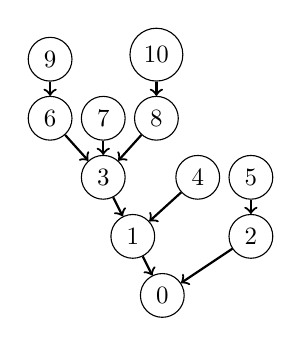
\begin{tikzpicture}[scale=.5, anchor=south]
      \node[circle, scale=0.9, draw] (tid0) at (3,1.5){0};
      \node[circle, scale=0.9, draw] (tid1) at (2.25,3){1};
      \node[circle, scale=0.9, draw] (tid2) at (1.5,4.5){3};
      \node[circle, scale=0.9, draw] (tid7) at (0.15,6){6};
      \node[circle, scale=0.9, draw] (tid9) at (0.15,7.5){9};
      \draw[<-, thick](tid7) -- (tid9);
      \node[circle, scale=0.9, draw] (tid10) at (1.5,6){7};
      \draw[<-, thick](tid2) -- (tid7);
      \draw[<-, thick](tid2) -- (tid10);
      \node[circle, scale=0.9, draw] (tid3) at (3.9,4.5){4};
      \node[circle, scale=0.9, draw] (tid5) at (2.85,6){8};
      \node[circle, scale=0.9, draw] (tid6) at (2.85,7.5){10
};
      \draw[<-, thick](tid5) -- (tid6);
      \draw[<-, thick](tid2) -- (tid5);
      \draw[<-, thick](tid1) -- (tid2);
      \draw[<-, thick](tid1) -- (tid3);
      \node[circle, scale=0.9, draw] (tid4) at (5.25,3){2};
      \node[circle, scale=0.9, draw] (tid8) at (5.25,4.5){5};
      \draw[<-, thick](tid4) -- (tid8);
      \draw[<-, thick](tid0) -- (tid1);
      \draw[<-, thick](tid0) -- (tid4);
    \end{tikzpicture}
  \end{center}
\end{frame}

\subsection{Schedules}
\label{sec:schedules}

\begin{frame}
  \frametitle{Schedules and snapshots}
  \begin{block}{Schedules}
    \begin{itemize}
    \item Describes the order of tasks
    \item Our scenario: non-deterministic (task times are random)
    \item Scheduling \emph{strategy} influences expected make span
    \end{itemize}
  \end{block}
  \begin{block}{Snapshots}
    \begin{itemize}
    \item States of a schedule
    \item Consist of current intree and the set of scheduled tasks
    % \item A schedule can be visualized by a snapshot DAG
    \end{itemize}
  \end{block}
\end{frame}

\begin{frame}
  \frametitle{Epected run time}
  \begin{itemize}
  \item $r$ tasks currently scheduled
  \item Each of these tasks is the first to finish with probability $\frac{1}{r}$
  \item Compute run time recursively (task times memoryless)
    \begin{itemize}
    \item Expected time for fastest task $\frac{1}{r}$
    \item Weighted expected time for successive snapshots
    \end{itemize}
  \end{itemize}
\end{frame}

\begin{frame}
  \frametitle{Schedule visualization}
  \only<1>{
    \begin{center}
      \renewcommand{\leveltopI}{-15cm + \leveltop}
\renewcommand{\leveltopII}{-15cm + \leveltopI}
\renewcommand{\leveltopIII}{-16cm + \leveltopII}
\renewcommand{\leveltopIIII}{-12cm + \leveltopIII}
\renewcommand{\leveltopIIIII}{-12cm + \leveltopIIII}
\renewcommand{\leveltopIIIIII}{-12cm + \leveltopIIIII}
\renewcommand{\leveltopIIIIIII}{-12cm + \leveltopIIIIII}
\renewcommand{\leveltopIIIIIIII}{-12cm + \leveltopIIIIIII}
\renewcommand{\leveltopIIIIIIIII}{-12cm + \leveltopIIIIIIII}
\renewcommand{\leveltopIIIIIIIIII}{-12cm + \leveltopIIIIIIIII}
\renewcommand{\leveltopIIIIIIIIIII}{-12cm + \leveltopIIIIIIIIII}
\begin{tikzpicture}[scale=.13333, anchor=south]
  % legende
  \filldraw[dashed,fill=gray!10!white] (-20, -30) rectangle +(36.5, 12);
  % \draw[dashed] (-30, -13) -- +(60, 0);
  % \draw[dashed] (-30, -24) -- +(60, 0);
  % \node at (10, -21) {Intermediate snapshots};
  \begin{scope}[yshift=\leveltopI cm]
    \matrix (line1)[column sep=0.5cm, ampersand replacement=\&] {
      \node[draw=black, rectangle split,  rectangle split parts=1] (sn0x17d67b0){
        \begin{tikzpicture}[scale=.13333]
          \node[circle, scale=0.5, fill] (tid0) at (4.5,1.5){};
          \node[circle, scale=0.5, fill] (tid2) at (2.25,3){};
          \node[circle, scale=0.5, fill, task_scheduled] (tid4) at (2.25,4.5){};
          \draw[](tid2) -- (tid4);
          \node[circle, scale=0.5, fill] (tid3) at (6,3){};
          \node[circle, scale=0.5, fill] (tid5) at (3.75,4.5){};
          \node[circle, scale=0.5, fill] (tid6) at (5.25,4.5){};
          \node[circle, scale=0.5, fill] (tid7) at (7.5,4.5){};
          \node[circle, scale=0.5, fill] (tid8) at (6.75,6){};
          \node[circle, scale=0.5, fill] (tid9) at (8.25,6){};
          \node[circle, scale=0.5, fill, task_scheduled] (tid10) at (8.25,7.5){};
          \draw[](tid9) -- (tid10);
          \draw[](tid7) -- (tid8);
          \draw[](tid7) -- (tid9);
          \draw[](tid3) -- (tid5);
          \draw[](tid3) -- (tid6);
          \draw[](tid3) -- (tid7);
          \draw[](tid0) -- (tid2);
          \draw[](tid0) -- (tid3);
        \end{tikzpicture}
      }
      ;
      \& 
      \\
    };
  \end{scope}
  \begin{scope}[yshift=\leveltopII cm]
    \matrix (line2)[column sep=0.5cm, ampersand replacement=\&] {
      \node[draw=black, rectangle split,  rectangle split parts=1] (sn0x17d65a0){
        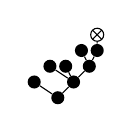
\begin{tikzpicture}[scale=.13333]
          \node[circle, scale=0.5, fill] (tid0) at (4.5,1.5){};
          \node[circle, scale=0.5, fill] (tid2) at (2.25,3){};
          \node[circle, scale=0.5, fill] (tid3) at (6,3){};
          \node[circle, scale=0.5, fill] (tid5) at (3.75,4.5){};
          \node[circle, scale=0.5, fill] (tid6) at (5.25,4.5){};
          \node[circle, scale=0.5, fill] (tid7) at (7.5,4.5){};
          \node[circle, scale=0.5, fill] (tid8) at (6.75,6){};
          \node[circle, scale=0.5, fill] (tid9) at (8.25,6){};
          \node[circle, scale=0.5, fill, task_scheduled] (tid10) at (8.25,7.5){};
          \draw[](tid9) -- (tid10);
          \draw[](tid7) -- (tid8);
          \draw[](tid7) -- (tid9);
          \draw[](tid3) -- (tid5);
          \draw[](tid3) -- (tid6);
          \draw[](tid3) -- (tid7);
          \draw[](tid0) -- (tid2);
          \draw[](tid0) -- (tid3);
        \end{tikzpicture}
      }
      ;
      \& 
      \node[minimum width=1cm]{};
      \&
      \node[draw=black, rectangle split,  rectangle split parts=1] (sn0x17d57c0){
        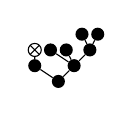
\begin{tikzpicture}[scale=.13333]
          \node[circle, scale=0.5, fill] (tid0) at (4.5,1.5){};
          \node[circle, scale=0.5, fill] (tid2) at (2.25,3){};
          \node[circle, scale=0.5, fill, task_scheduled] (tid4) at (2.25,4.5){};
          \draw[](tid2) -- (tid4);
          \node[circle, scale=0.5, fill] (tid3) at (6,3){};
          \node[circle, scale=0.5, fill] (tid5) at (3.75,4.5){};
          \node[circle, scale=0.5, fill] (tid6) at (5.25,4.5){};
          \node[circle, scale=0.5, fill] (tid7) at (7.5,4.5){};
          \node[circle, scale=0.5, fill] (tid8) at (6.75,6){};
          \node[circle, scale=0.5, fill] (tid9) at (8.25,6){};
          \draw[](tid7) -- (tid8);
          \draw[](tid7) -- (tid9);
          \draw[](tid3) -- (tid5);
          \draw[](tid3) -- (tid6);
          \draw[](tid3) -- (tid7);
          \draw[](tid0) -- (tid2);
          \draw[](tid0) -- (tid3);
        \end{tikzpicture}
      }
      ;
      \& 
      \\
    };
  \end{scope}
  \begin{scope}[yshift=\leveltopIII cm]
    \matrix (line3)[column sep=0.5cm, ampersand replacement=\&] {
      \node[draw=black, rectangle split,  rectangle split parts=1] (sn0x17d55b0){
        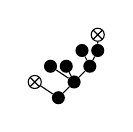
\begin{tikzpicture}[scale=.13333]
          \node[circle, scale=0.5, fill] (tid0) at (4.5,1.5){};
          \node[circle, scale=0.5, fill, task_scheduled] (tid2) at (2.25,3){};
          \node[circle, scale=0.5, fill] (tid3) at (6,3){};
          \node[circle, scale=0.5, fill] (tid5) at (3.75,4.5){};
          \node[circle, scale=0.5, fill] (tid6) at (5.25,4.5){};
          \node[circle, scale=0.5, fill] (tid7) at (7.5,4.5){};
          \node[circle, scale=0.5, fill] (tid8) at (6.75,6){};
          \node[circle, scale=0.5, fill] (tid9) at (8.25,6){};
          \node[circle, scale=0.5, fill, task_scheduled] (tid10) at (8.25,7.5){};
          \draw[](tid9) -- (tid10);
          \draw[](tid7) -- (tid8);
          \draw[](tid7) -- (tid9);
          \draw[](tid3) -- (tid5);
          \draw[](tid3) -- (tid6);
          \draw[](tid3) -- (tid7);
          \draw[](tid0) -- (tid2);
          \draw[](tid0) -- (tid3);
        \end{tikzpicture}
      }
      ;
      \& 
      \node[draw=black, rectangle split,  rectangle split parts=1] (sn0x17d6160){
        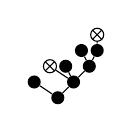
\begin{tikzpicture}[scale=.13333]
          \node[circle, scale=0.5, fill] (tid0) at (4.5,1.5){};
          \node[circle, scale=0.5, fill] (tid2) at (2.25,3){};
          \node[circle, scale=0.5, fill] (tid3) at (6,3){};
          \node[circle, scale=0.5, fill, task_scheduled] (tid5) at (3.75,4.5){};
          \node[circle, scale=0.5, fill] (tid6) at (5.25,4.5){};
          \node[circle, scale=0.5, fill] (tid7) at (7.5,4.5){};
          \node[circle, scale=0.5, fill] (tid8) at (6.75,6){};
          \node[circle, scale=0.5, fill] (tid9) at (8.25,6){};
          \node[circle, scale=0.5, fill, task_scheduled] (tid10) at (8.25,7.5){};
          \draw[](tid9) -- (tid10);
          \draw[](tid7) -- (tid8);
          \draw[](tid7) -- (tid9);
          \draw[](tid3) -- (tid5);
          \draw[](tid3) -- (tid6);
          \draw[](tid3) -- (tid7);
          \draw[](tid0) -- (tid2);
          \draw[](tid0) -- (tid3);
        \end{tikzpicture}
      }
      ;
      \& 
      \node[draw=black, rectangle split,  rectangle split parts=1] (sn0x17d5380){
        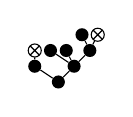
\begin{tikzpicture}[scale=.13333]
          \node[circle, scale=0.5, fill] (tid0) at (4.5,1.5){};
          \node[circle, scale=0.5, fill] (tid2) at (2.25,3){};
          \node[circle, scale=0.5, fill, task_scheduled] (tid4) at (2.25,4.5){};
          \draw[](tid2) -- (tid4);
          \node[circle, scale=0.5, fill] (tid3) at (6,3){};
          \node[circle, scale=0.5, fill] (tid5) at (3.75,4.5){};
          \node[circle, scale=0.5, fill] (tid6) at (5.25,4.5){};
          \node[circle, scale=0.5, fill] (tid7) at (7.5,4.5){};
          \node[circle, scale=0.5, fill] (tid8) at (6.75,6){};
          \node[circle, scale=0.5, fill, task_scheduled] (tid9) at (8.25,6){};
          \draw[](tid7) -- (tid8);
          \draw[](tid7) -- (tid9);
          \draw[](tid3) -- (tid5);
          \draw[](tid3) -- (tid6);
          \draw[](tid3) -- (tid7);
          \draw[](tid0) -- (tid2);
          \draw[](tid0) -- (tid3);
        \end{tikzpicture}
      }
      ;
      \& 
      \node[draw=black, rectangle split,  rectangle split parts=1] (sn0x17d2f50){
        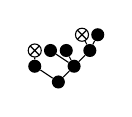
\begin{tikzpicture}[scale=.13333]
          \node[circle, scale=0.5, fill] (tid0) at (4.5,1.5){};
          \node[circle, scale=0.5, fill] (tid2) at (2.25,3){};
          \node[circle, scale=0.5, fill, task_scheduled] (tid4) at (2.25,4.5){};
          \draw[](tid2) -- (tid4);
          \node[circle, scale=0.5, fill] (tid3) at (6,3){};
          \node[circle, scale=0.5, fill] (tid5) at (3.75,4.5){};
          \node[circle, scale=0.5, fill] (tid6) at (5.25,4.5){};
          \node[circle, scale=0.5, fill] (tid7) at (7.5,4.5){};
          \node[circle, scale=0.5, fill, task_scheduled] (tid8) at (6.75,6){};
          \node[circle, scale=0.5, fill] (tid9) at (8.25,6){};
          \draw[](tid7) -- (tid8);
          \draw[](tid7) -- (tid9);
          \draw[](tid3) -- (tid5);
          \draw[](tid3) -- (tid6);
          \draw[](tid3) -- (tid7);
          \draw[](tid0) -- (tid2);
          \draw[](tid0) -- (tid3);
        \end{tikzpicture}
      }
      ;
      \& 
      \node[draw=black, rectangle split,  rectangle split parts=1] (sn0x17d3a00){
        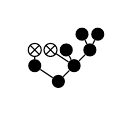
\begin{tikzpicture}[scale=.13333]
          \node[circle, scale=0.5, fill] (tid0) at (4.5,1.5){};
          \node[circle, scale=0.5, fill] (tid2) at (2.25,3){};
          \node[circle, scale=0.5, fill, task_scheduled] (tid4) at (2.25,4.5){};
          \draw[](tid2) -- (tid4);
          \node[circle, scale=0.5, fill] (tid3) at (6,3){};
          \node[circle, scale=0.5, fill, task_scheduled] (tid5) at (3.75,4.5){};
          \node[circle, scale=0.5, fill] (tid6) at (5.25,4.5){};
          \node[circle, scale=0.5, fill] (tid7) at (7.5,4.5){};
          \node[circle, scale=0.5, fill] (tid8) at (6.75,6){};
          \node[circle, scale=0.5, fill] (tid9) at (8.25,6){};
          \draw[](tid7) -- (tid8);
          \draw[](tid7) -- (tid9);
          \draw[](tid3) -- (tid5);
          \draw[](tid3) -- (tid6);
          \draw[](tid3) -- (tid7);
          \draw[](tid0) -- (tid2);
          \draw[](tid0) -- (tid3);
        \end{tikzpicture}
      }
      ;
      \& 
      \\
    };
  \end{scope}
  \draw (sn0x17d67b0.south) -- node[xshift=.4cm]{$0.5$} (sn0x17d57c0.north);
  \draw (sn0x17d67b0.south) -- node[left, yshift=.2cm]{$0.5$} (sn0x17d65a0.north);
  \draw (sn0x17d65a0.south) -- node[right]{$0.8$} (sn0x17d6160.north);
  \draw (sn0x17d65a0.south) -- node[left, xshift=-.25cm]{$0.2$} (sn0x17d55b0.north);
  \draw (sn0x17d57c0.south) -- node[right, xshift=.25]{$0.2$} (sn0x17d2f50.north);
  \draw (sn0x17d57c0.south) -- node[left, xshift=-3]{$0.4$} (sn0x17d5380.north);
  \draw (sn0x17d57c0.south) -- node[right, xshift=5]{$0.4$} (sn0x17d3a00.north);
\end{tikzpicture} % with intermediate snaps
    \end{center}
  }
  \only<2>{
    \begin{center}
      \renewcommand{\leveltopI}{-25cm + \leveltop}
\renewcommand{\leveltopII}{-25cm + \leveltopI}
\renewcommand{\leveltopIII}{-16cm + \leveltopII}
\renewcommand{\leveltopIIII}{-12cm + \leveltopIII}
\renewcommand{\leveltopIIIII}{-12cm + \leveltopIIII}
\renewcommand{\leveltopIIIIII}{-12cm + \leveltopIIIII}
\renewcommand{\leveltopIIIIIII}{-12cm + \leveltopIIIIII}
\renewcommand{\leveltopIIIIIIII}{-12cm + \leveltopIIIIIII}
\renewcommand{\leveltopIIIIIIIII}{-12cm + \leveltopIIIIIIII}
\renewcommand{\leveltopIIIIIIIIII}{-12cm + \leveltopIIIIIIIII}
\renewcommand{\leveltopIIIIIIIIIII}{-12cm + \leveltopIIIIIIIIII}
\begin{tikzpicture}[scale=.13333, anchor=south]
  % legende
  %\filldraw[dashed,fill=gray!10!white] (-20, -30) rectangle +(36.5, 12);
  % \draw[dashed] (-30, -13) -- +(60, 0);
  % \draw[dashed] (-30, -24) -- +(60, 0);
  % \node at (10, -21) {Intermediate snapshots};
  \begin{scope}[yshift=\leveltopI cm]
    \matrix (line1)[column sep=0.5cm, ampersand replacement=\&] {
      \node[draw=black, rectangle split,  rectangle split parts=1] (sn0x17d67b0){
        \begin{tikzpicture}[scale=.13333]
          \node[circle, scale=0.5, fill] (tid0) at (4.5,1.5){};
          \node[circle, scale=0.5, fill] (tid2) at (2.25,3){};
          \node[circle, scale=0.5, fill, task_scheduled] (tid4) at (2.25,4.5){};
          \draw[](tid2) -- (tid4);
          \node[circle, scale=0.5, fill] (tid3) at (6,3){};
          \node[circle, scale=0.5, fill] (tid5) at (3.75,4.5){};
          \node[circle, scale=0.5, fill] (tid6) at (5.25,4.5){};
          \node[circle, scale=0.5, fill] (tid7) at (7.5,4.5){};
          \node[circle, scale=0.5, fill] (tid8) at (6.75,6){};
          \node[circle, scale=0.5, fill] (tid9) at (8.25,6){};
          \node[circle, scale=0.5, fill, task_scheduled] (tid10) at (8.25,7.5){};
          \draw[](tid9) -- (tid10);
          \draw[](tid7) -- (tid8);
          \draw[](tid7) -- (tid9);
          \draw[](tid3) -- (tid5);
          \draw[](tid3) -- (tid6);
          \draw[](tid3) -- (tid7);
          \draw[](tid0) -- (tid2);
          \draw[](tid0) -- (tid3);
        \end{tikzpicture}
      }
      ;
      \& 
      \\
    };
  \end{scope}
  \begin{scope}[yshift=\leveltopII cm]
    \matrix (line2)[column sep=.5cm, ampersand replacement=\&] {
      \node[draw=black, rectangle split,  rectangle split parts=1] (sn0x17d55b0){
        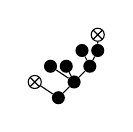
\begin{tikzpicture}[scale=.13333]
          \node[circle, scale=0.5, fill] (tid0) at (4.5,1.5){};
          \node[circle, scale=0.5, fill, task_scheduled] (tid2) at (2.25,3){};
          \node[circle, scale=0.5, fill] (tid3) at (6,3){};
          \node[circle, scale=0.5, fill] (tid5) at (3.75,4.5){};
          \node[circle, scale=0.5, fill] (tid6) at (5.25,4.5){};
          \node[circle, scale=0.5, fill] (tid7) at (7.5,4.5){};
          \node[circle, scale=0.5, fill] (tid8) at (6.75,6){};
          \node[circle, scale=0.5, fill] (tid9) at (8.25,6){};
          \node[circle, scale=0.5, fill, task_scheduled] (tid10) at (8.25,7.5){};
          \draw[](tid9) -- (tid10);
          \draw[](tid7) -- (tid8);
          \draw[](tid7) -- (tid9);
          \draw[](tid3) -- (tid5);
          \draw[](tid3) -- (tid6);
          \draw[](tid3) -- (tid7);
          \draw[](tid0) -- (tid2);
          \draw[](tid0) -- (tid3);
        \end{tikzpicture}
      }
      ;
      \& 
      \node[draw=black, rectangle split,  rectangle split parts=1] (sn0x17d6160){
        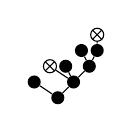
\begin{tikzpicture}[scale=.13333]
          \node[circle, scale=0.5, fill] (tid0) at (4.5,1.5){};
          \node[circle, scale=0.5, fill] (tid2) at (2.25,3){};
          \node[circle, scale=0.5, fill] (tid3) at (6,3){};
          \node[circle, scale=0.5, fill, task_scheduled] (tid5) at (3.75,4.5){};
          \node[circle, scale=0.5, fill] (tid6) at (5.25,4.5){};
          \node[circle, scale=0.5, fill] (tid7) at (7.5,4.5){};
          \node[circle, scale=0.5, fill] (tid8) at (6.75,6){};
          \node[circle, scale=0.5, fill] (tid9) at (8.25,6){};
          \node[circle, scale=0.5, fill, task_scheduled] (tid10) at (8.25,7.5){};
          \draw[](tid9) -- (tid10);
          \draw[](tid7) -- (tid8);
          \draw[](tid7) -- (tid9);
          \draw[](tid3) -- (tid5);
          \draw[](tid3) -- (tid6);
          \draw[](tid3) -- (tid7);
          \draw[](tid0) -- (tid2);
          \draw[](tid0) -- (tid3);
        \end{tikzpicture}
      }
      ;
      \& 
      \node[draw=black, rectangle split,  rectangle split parts=1] (sn0x17d5380){
        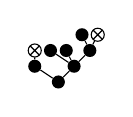
\begin{tikzpicture}[scale=.13333]
          \node[circle, scale=0.5, fill] (tid0) at (4.5,1.5){};
          \node[circle, scale=0.5, fill] (tid2) at (2.25,3){};
          \node[circle, scale=0.5, fill, task_scheduled] (tid4) at (2.25,4.5){};
          \draw[](tid2) -- (tid4);
          \node[circle, scale=0.5, fill] (tid3) at (6,3){};
          \node[circle, scale=0.5, fill] (tid5) at (3.75,4.5){};
          \node[circle, scale=0.5, fill] (tid6) at (5.25,4.5){};
          \node[circle, scale=0.5, fill] (tid7) at (7.5,4.5){};
          \node[circle, scale=0.5, fill] (tid8) at (6.75,6){};
          \node[circle, scale=0.5, fill, task_scheduled] (tid9) at (8.25,6){};
          \draw[](tid7) -- (tid8);
          \draw[](tid7) -- (tid9);
          \draw[](tid3) -- (tid5);
          \draw[](tid3) -- (tid6);
          \draw[](tid3) -- (tid7);
          \draw[](tid0) -- (tid2);
          \draw[](tid0) -- (tid3);
        \end{tikzpicture}
      }
      ;
      \& 
      \node[draw=black, rectangle split,  rectangle split parts=1] (sn0x17d2f50){
        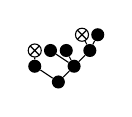
\begin{tikzpicture}[scale=.13333]
          \node[circle, scale=0.5, fill] (tid0) at (4.5,1.5){};
          \node[circle, scale=0.5, fill] (tid2) at (2.25,3){};
          \node[circle, scale=0.5, fill, task_scheduled] (tid4) at (2.25,4.5){};
          \draw[](tid2) -- (tid4);
          \node[circle, scale=0.5, fill] (tid3) at (6,3){};
          \node[circle, scale=0.5, fill] (tid5) at (3.75,4.5){};
          \node[circle, scale=0.5, fill] (tid6) at (5.25,4.5){};
          \node[circle, scale=0.5, fill] (tid7) at (7.5,4.5){};
          \node[circle, scale=0.5, fill, task_scheduled] (tid8) at (6.75,6){};
          \node[circle, scale=0.5, fill] (tid9) at (8.25,6){};
          \draw[](tid7) -- (tid8);
          \draw[](tid7) -- (tid9);
          \draw[](tid3) -- (tid5);
          \draw[](tid3) -- (tid6);
          \draw[](tid3) -- (tid7);
          \draw[](tid0) -- (tid2);
          \draw[](tid0) -- (tid3);
        \end{tikzpicture}
      }
      ;
      \& 
      \node[draw=black, rectangle split,  rectangle split parts=1] (sn0x17d3a00){
        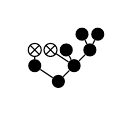
\begin{tikzpicture}[scale=.13333]
          \node[circle, scale=0.5, fill] (tid0) at (4.5,1.5){};
          \node[circle, scale=0.5, fill] (tid2) at (2.25,3){};
          \node[circle, scale=0.5, fill, task_scheduled] (tid4) at (2.25,4.5){};
          \draw[](tid2) -- (tid4);
          \node[circle, scale=0.5, fill] (tid3) at (6,3){};
          \node[circle, scale=0.5, fill, task_scheduled] (tid5) at (3.75,4.5){};
          \node[circle, scale=0.5, fill] (tid6) at (5.25,4.5){};
          \node[circle, scale=0.5, fill] (tid7) at (7.5,4.5){};
          \node[circle, scale=0.5, fill] (tid8) at (6.75,6){};
          \node[circle, scale=0.5, fill] (tid9) at (8.25,6){};
          \draw[](tid7) -- (tid8);
          \draw[](tid7) -- (tid9);
          \draw[](tid3) -- (tid5);
          \draw[](tid3) -- (tid6);
          \draw[](tid3) -- (tid7);
          \draw[](tid0) -- (tid2);
          \draw[](tid0) -- (tid3);
        \end{tikzpicture}
      }
      ;
      \& 
      \\
    };
  \end{scope}
  \draw (sn0x17d67b0.south) -- node[left]{$0.4$} (sn0x17d6160.north);
  \draw (sn0x17d67b0.south) -- node[left, xshift=-.25cm]{$0.1$} (sn0x17d55b0.north);
  \draw (sn0x17d67b0.south) -- node[right, xshift=.25]{$0.1$} (sn0x17d2f50.north);
  \draw (sn0x17d67b0.south) -- node[left]{$0.2$} (sn0x17d5380.north);
  \draw (sn0x17d67b0.south) -- node[right, xshift=5]{$0.2$} (sn0x17d3a00.north);
\end{tikzpicture} % without intermediate snaps
    \end{center}
  }
  \only<3>{
    \begin{center}
      \renewcommand{\leveltopI}{-25cm + \leveltop}
\renewcommand{\leveltopII}{-25cm + \leveltopI}
\renewcommand{\leveltopIII}{-16cm + \leveltopII}
\renewcommand{\leveltopIIII}{-12cm + \leveltopIII}
\renewcommand{\leveltopIIIII}{-12cm + \leveltopIIII}
\renewcommand{\leveltopIIIIII}{-12cm + \leveltopIIIII}
\renewcommand{\leveltopIIIIIII}{-12cm + \leveltopIIIIII}
\renewcommand{\leveltopIIIIIIII}{-12cm + \leveltopIIIIIII}
\renewcommand{\leveltopIIIIIIIII}{-12cm + \leveltopIIIIIIII}
\renewcommand{\leveltopIIIIIIIIII}{-12cm + \leveltopIIIIIIIII}
\renewcommand{\leveltopIIIIIIIIIII}{-12cm + \leveltopIIIIIIIIII}
\begin{tikzpicture}[scale=.13333, anchor=south]
  % legende
  %\filldraw[dashed,fill=gray!10!white] (-20, -30) rectangle +(36.5, 12);
  % \draw[dashed] (-30, -13) -- +(60, 0);
  % \draw[dashed] (-30, -24) -- +(60, 0);
  % \node at (10, -21) {Intermediate snapshots};
  \begin{scope}[yshift=\leveltopI cm]
    \matrix (line1)[column sep=0.5cm, ampersand replacement=\&] {
      \node[draw=black, rectangle split,  rectangle split parts=2] (sn0x17d67b0){
        \begin{tikzpicture}[scale=.13333]
          \node[circle, scale=0.5, fill] (tid0) at (4.5,1.5){};
          \node[circle, scale=0.5, fill] (tid2) at (2.25,3){};
          \node[circle, scale=0.5, fill, task_scheduled] (tid4) at (2.25,4.5){};
          \draw[](tid2) -- (tid4);
          \node[circle, scale=0.5, fill] (tid3) at (6,3){};
          \node[circle, scale=0.5, fill] (tid5) at (3.75,4.5){};
          \node[circle, scale=0.5, fill] (tid6) at (5.25,4.5){};
          \node[circle, scale=0.5, fill] (tid7) at (7.5,4.5){};
          \node[circle, scale=0.5, fill] (tid8) at (6.75,6){};
          \node[circle, scale=0.5, fill] (tid9) at (8.25,6){};
          \node[circle, scale=0.5, fill, task_scheduled] (tid10) at (8.25,7.5){};
          \draw[](tid9) -- (tid10);
          \draw[](tid7) -- (tid8);
          \draw[](tid7) -- (tid9);
          \draw[](tid3) -- (tid5);
          \draw[](tid3) -- (tid6);
          \draw[](tid3) -- (tid7);
          \draw[](tid0) -- (tid2);
          \draw[](tid0) -- (tid3);
        \end{tikzpicture}
        \nodepart{second}
        \footnotesize{10\ 40\ 20\ 10\ 20}
      }
      ;
      \& 
      \\
    };
  \end{scope}
  \begin{scope}[yshift=\leveltopII cm]
    \matrix (line2)[column sep=.5cm, ampersand replacement=\&] {
      \node[draw=black, rectangle split,  rectangle split parts=1] (sn0x17d55b0){
        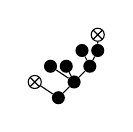
\begin{tikzpicture}[scale=.13333]
          \node[circle, scale=0.5, fill] (tid0) at (4.5,1.5){};
          \node[circle, scale=0.5, fill, task_scheduled] (tid2) at (2.25,3){};
          \node[circle, scale=0.5, fill] (tid3) at (6,3){};
          \node[circle, scale=0.5, fill] (tid5) at (3.75,4.5){};
          \node[circle, scale=0.5, fill] (tid6) at (5.25,4.5){};
          \node[circle, scale=0.5, fill] (tid7) at (7.5,4.5){};
          \node[circle, scale=0.5, fill] (tid8) at (6.75,6){};
          \node[circle, scale=0.5, fill] (tid9) at (8.25,6){};
          \node[circle, scale=0.5, fill, task_scheduled] (tid10) at (8.25,7.5){};
          \draw[](tid9) -- (tid10);
          \draw[](tid7) -- (tid8);
          \draw[](tid7) -- (tid9);
          \draw[](tid3) -- (tid5);
          \draw[](tid3) -- (tid6);
          \draw[](tid3) -- (tid7);
          \draw[](tid0) -- (tid2);
          \draw[](tid0) -- (tid3);
        \end{tikzpicture}
      }
      ;
      \& 
      \node[draw=black, rectangle split,  rectangle split parts=1] (sn0x17d6160){
        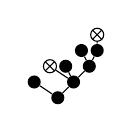
\begin{tikzpicture}[scale=.13333]
          \node[circle, scale=0.5, fill] (tid0) at (4.5,1.5){};
          \node[circle, scale=0.5, fill] (tid2) at (2.25,3){};
          \node[circle, scale=0.5, fill] (tid3) at (6,3){};
          \node[circle, scale=0.5, fill, task_scheduled] (tid5) at (3.75,4.5){};
          \node[circle, scale=0.5, fill] (tid6) at (5.25,4.5){};
          \node[circle, scale=0.5, fill] (tid7) at (7.5,4.5){};
          \node[circle, scale=0.5, fill] (tid8) at (6.75,6){};
          \node[circle, scale=0.5, fill] (tid9) at (8.25,6){};
          \node[circle, scale=0.5, fill, task_scheduled] (tid10) at (8.25,7.5){};
          \draw[](tid9) -- (tid10);
          \draw[](tid7) -- (tid8);
          \draw[](tid7) -- (tid9);
          \draw[](tid3) -- (tid5);
          \draw[](tid3) -- (tid6);
          \draw[](tid3) -- (tid7);
          \draw[](tid0) -- (tid2);
          \draw[](tid0) -- (tid3);
        \end{tikzpicture}
      }
      ;
      \& 
      \node[draw=black, rectangle split,  rectangle split parts=1] (sn0x17d5380){
        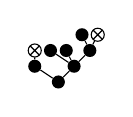
\begin{tikzpicture}[scale=.13333]
          \node[circle, scale=0.5, fill] (tid0) at (4.5,1.5){};
          \node[circle, scale=0.5, fill] (tid2) at (2.25,3){};
          \node[circle, scale=0.5, fill, task_scheduled] (tid4) at (2.25,4.5){};
          \draw[](tid2) -- (tid4);
          \node[circle, scale=0.5, fill] (tid3) at (6,3){};
          \node[circle, scale=0.5, fill] (tid5) at (3.75,4.5){};
          \node[circle, scale=0.5, fill] (tid6) at (5.25,4.5){};
          \node[circle, scale=0.5, fill] (tid7) at (7.5,4.5){};
          \node[circle, scale=0.5, fill] (tid8) at (6.75,6){};
          \node[circle, scale=0.5, fill, task_scheduled] (tid9) at (8.25,6){};
          \draw[](tid7) -- (tid8);
          \draw[](tid7) -- (tid9);
          \draw[](tid3) -- (tid5);
          \draw[](tid3) -- (tid6);
          \draw[](tid3) -- (tid7);
          \draw[](tid0) -- (tid2);
          \draw[](tid0) -- (tid3);
        \end{tikzpicture}
      }
      ;
      \& 
      \node[draw=black, rectangle split,  rectangle split parts=1] (sn0x17d2f50){
        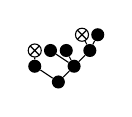
\begin{tikzpicture}[scale=.13333]
          \node[circle, scale=0.5, fill] (tid0) at (4.5,1.5){};
          \node[circle, scale=0.5, fill] (tid2) at (2.25,3){};
          \node[circle, scale=0.5, fill, task_scheduled] (tid4) at (2.25,4.5){};
          \draw[](tid2) -- (tid4);
          \node[circle, scale=0.5, fill] (tid3) at (6,3){};
          \node[circle, scale=0.5, fill] (tid5) at (3.75,4.5){};
          \node[circle, scale=0.5, fill] (tid6) at (5.25,4.5){};
          \node[circle, scale=0.5, fill] (tid7) at (7.5,4.5){};
          \node[circle, scale=0.5, fill, task_scheduled] (tid8) at (6.75,6){};
          \node[circle, scale=0.5, fill] (tid9) at (8.25,6){};
          \draw[](tid7) -- (tid8);
          \draw[](tid7) -- (tid9);
          \draw[](tid3) -- (tid5);
          \draw[](tid3) -- (tid6);
          \draw[](tid3) -- (tid7);
          \draw[](tid0) -- (tid2);
          \draw[](tid0) -- (tid3);
        \end{tikzpicture}
      }
      ;
      \& 
      \node[draw=black, rectangle split,  rectangle split parts=1] (sn0x17d3a00){
        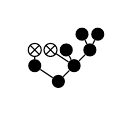
\begin{tikzpicture}[scale=.13333]
          \node[circle, scale=0.5, fill] (tid0) at (4.5,1.5){};
          \node[circle, scale=0.5, fill] (tid2) at (2.25,3){};
          \node[circle, scale=0.5, fill, task_scheduled] (tid4) at (2.25,4.5){};
          \draw[](tid2) -- (tid4);
          \node[circle, scale=0.5, fill] (tid3) at (6,3){};
          \node[circle, scale=0.5, fill, task_scheduled] (tid5) at (3.75,4.5){};
          \node[circle, scale=0.5, fill] (tid6) at (5.25,4.5){};
          \node[circle, scale=0.5, fill] (tid7) at (7.5,4.5){};
          \node[circle, scale=0.5, fill] (tid8) at (6.75,6){};
          \node[circle, scale=0.5, fill] (tid9) at (8.25,6){};
          \draw[](tid7) -- (tid8);
          \draw[](tid7) -- (tid9);
          \draw[](tid3) -- (tid5);
          \draw[](tid3) -- (tid6);
          \draw[](tid3) -- (tid7);
          \draw[](tid0) -- (tid2);
          \draw[](tid0) -- (tid3);
        \end{tikzpicture}
      }
      ;
      \& 
      \\
    };
  \end{scope}
  \draw (sn0x17d67b0.south) -- (sn0x17d6160.north);
  \draw (sn0x17d67b0.south) -- (sn0x17d55b0.north);
  \draw (sn0x17d67b0.south) -- (sn0x17d2f50.north);
  \draw (sn0x17d67b0.south) -- (sn0x17d5380.north);
  \draw (sn0x17d67b0.south) -- (sn0x17d3a00.north);
\end{tikzpicture} % compressed form
    \end{center}
  }
  \only<4>{
    \begin{center}
      \renewcommand{\leveltopI}{-25cm + \leveltop}
\renewcommand{\leveltopII}{-25cm + \leveltopI}
\renewcommand{\leveltopIII}{-16cm + \leveltopII}
\renewcommand{\leveltopIIII}{-12cm + \leveltopIII}
\renewcommand{\leveltopIIIII}{-12cm + \leveltopIIII}
\renewcommand{\leveltopIIIIII}{-12cm + \leveltopIIIII}
\renewcommand{\leveltopIIIIIII}{-12cm + \leveltopIIIIII}
\renewcommand{\leveltopIIIIIIII}{-12cm + \leveltopIIIIIII}
\renewcommand{\leveltopIIIIIIIII}{-12cm + \leveltopIIIIIIII}
\renewcommand{\leveltopIIIIIIIIII}{-12cm + \leveltopIIIIIIIII}
\renewcommand{\leveltopIIIIIIIIIII}{-12cm + \leveltopIIIIIIIIII}
\begin{tikzpicture}[scale=.13333, anchor=south]
  % legende
  %\filldraw[dashed,fill=gray!10!white] (-20, -30) rectangle +(36.5, 12);
  % \draw[dashed] (-30, -13) -- +(60, 0);
  % \draw[dashed] (-30, -24) -- +(60, 0);
  % \node at (10, -21) {Intermediate snapshots};
  \begin{scope}[yshift=\leveltopI cm]
    \matrix (line1)[column sep=0.5cm, ampersand replacement=\&] {
      \node[draw=black, rectangle split,  rectangle split parts=3] (sn0x17d67b0){
        \begin{tikzpicture}[scale=.13333]
          \node[circle, scale=0.5, fill] (tid0) at (4.5,1.5){};
          \node[circle, scale=0.5, fill] (tid2) at (2.25,3){};
          \node[circle, scale=0.5, fill, task_scheduled] (tid4) at (2.25,4.5){};
          \draw[](tid2) -- (tid4);
          \node[circle, scale=0.5, fill] (tid3) at (6,3){};
          \node[circle, scale=0.5, fill] (tid5) at (3.75,4.5){};
          \node[circle, scale=0.5, fill] (tid6) at (5.25,4.5){};
          \node[circle, scale=0.5, fill] (tid7) at (7.5,4.5){};
          \node[circle, scale=0.5, fill] (tid8) at (6.75,6){};
          \node[circle, scale=0.5, fill] (tid9) at (8.25,6){};
          \node[circle, scale=0.5, fill, task_scheduled] (tid10) at (8.25,7.5){};
          \draw[](tid9) -- (tid10);
          \draw[](tid7) -- (tid8);
          \draw[](tid7) -- (tid9);
          \draw[](tid3) -- (tid5);
          \draw[](tid3) -- (tid6);
          \draw[](tid3) -- (tid7);
          \draw[](tid0) -- (tid2);
          \draw[](tid0) -- (tid3);
        \end{tikzpicture}
        \nodepart{second}
        ? %6.43745
        \nodepart{third}
        \footnotesize{10\ 40\ 20\ 10\ 20}
      }
      ;
      \& 
      \\
    };
  \end{scope}
  \begin{scope}[yshift=\leveltopII cm]
    \matrix (line2)[column sep=.5cm, ampersand replacement=\&] {
      \node[draw=black, rectangle split,  rectangle split parts=2] (sn0x17d55b0){
        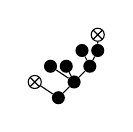
\begin{tikzpicture}[scale=.13333]
          \node[circle, scale=0.5, fill] (tid0) at (4.5,1.5){};
          \node[circle, scale=0.5, fill, task_scheduled] (tid2) at (2.25,3){};
          \node[circle, scale=0.5, fill] (tid3) at (6,3){};
          \node[circle, scale=0.5, fill] (tid5) at (3.75,4.5){};
          \node[circle, scale=0.5, fill] (tid6) at (5.25,4.5){};
          \node[circle, scale=0.5, fill] (tid7) at (7.5,4.5){};
          \node[circle, scale=0.5, fill] (tid8) at (6.75,6){};
          \node[circle, scale=0.5, fill] (tid9) at (8.25,6){};
          \node[circle, scale=0.5, fill, task_scheduled] (tid10) at (8.25,7.5){};
          \draw[](tid9) -- (tid10);
          \draw[](tid7) -- (tid8);
          \draw[](tid7) -- (tid9);
          \draw[](tid3) -- (tid5);
          \draw[](tid3) -- (tid6);
          \draw[](tid3) -- (tid7);
          \draw[](tid0) -- (tid2);
          \draw[](tid0) -- (tid3);
        \end{tikzpicture}
        \nodepart{second}
        6.1640
      }
      ;
      \& 
      \node[draw=black, rectangle split,  rectangle split parts=2] (sn0x17d6160){
        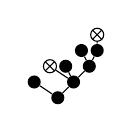
\begin{tikzpicture}[scale=.13333]
          \node[circle, scale=0.5, fill] (tid0) at (4.5,1.5){};
          \node[circle, scale=0.5, fill] (tid2) at (2.25,3){};
          \node[circle, scale=0.5, fill] (tid3) at (6,3){};
          \node[circle, scale=0.5, fill, task_scheduled] (tid5) at (3.75,4.5){};
          \node[circle, scale=0.5, fill] (tid6) at (5.25,4.5){};
          \node[circle, scale=0.5, fill] (tid7) at (7.5,4.5){};
          \node[circle, scale=0.5, fill] (tid8) at (6.75,6){};
          \node[circle, scale=0.5, fill] (tid9) at (8.25,6){};
          \node[circle, scale=0.5, fill, task_scheduled] (tid10) at (8.25,7.5){};
          \draw[](tid9) -- (tid10);
          \draw[](tid7) -- (tid8);
          \draw[](tid7) -- (tid9);
          \draw[](tid3) -- (tid5);
          \draw[](tid3) -- (tid6);
          \draw[](tid3) -- (tid7);
          \draw[](tid0) -- (tid2);
          \draw[](tid0) -- (tid3);
        \end{tikzpicture}
        \nodepart{second}
        5.9921
      }
      ;
      \& 
      \node[draw=black, rectangle split,  rectangle split parts=2] (sn0x17d5380){
        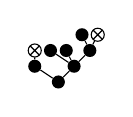
\begin{tikzpicture}[scale=.13333]
          \node[circle, scale=0.5, fill] (tid0) at (4.5,1.5){};
          \node[circle, scale=0.5, fill] (tid2) at (2.25,3){};
          \node[circle, scale=0.5, fill, task_scheduled] (tid4) at (2.25,4.5){};
          \draw[](tid2) -- (tid4);
          \node[circle, scale=0.5, fill] (tid3) at (6,3){};
          \node[circle, scale=0.5, fill] (tid5) at (3.75,4.5){};
          \node[circle, scale=0.5, fill] (tid6) at (5.25,4.5){};
          \node[circle, scale=0.5, fill] (tid7) at (7.5,4.5){};
          \node[circle, scale=0.5, fill] (tid8) at (6.75,6){};
          \node[circle, scale=0.5, fill, task_scheduled] (tid9) at (8.25,6){};
          \draw[](tid7) -- (tid8);
          \draw[](tid7) -- (tid9);
          \draw[](tid3) -- (tid5);
          \draw[](tid3) -- (tid6);
          \draw[](tid3) -- (tid7);
          \draw[](tid0) -- (tid2);
          \draw[](tid0) -- (tid3);
        \end{tikzpicture}
        \nodepart{second}
        5.8203
      }
      ;
      \& 
      \node[draw=black, rectangle split,  rectangle split parts=2] (sn0x17d2f50){
        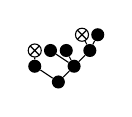
\begin{tikzpicture}[scale=.13333]
          \node[circle, scale=0.5, fill] (tid0) at (4.5,1.5){};
          \node[circle, scale=0.5, fill] (tid2) at (2.25,3){};
          \node[circle, scale=0.5, fill, task_scheduled] (tid4) at (2.25,4.5){};
          \draw[](tid2) -- (tid4);
          \node[circle, scale=0.5, fill] (tid3) at (6,3){};
          \node[circle, scale=0.5, fill] (tid5) at (3.75,4.5){};
          \node[circle, scale=0.5, fill] (tid6) at (5.25,4.5){};
          \node[circle, scale=0.5, fill] (tid7) at (7.5,4.5){};
          \node[circle, scale=0.5, fill, task_scheduled] (tid8) at (6.75,6){};
          \node[circle, scale=0.5, fill] (tid9) at (8.25,6){};
          \draw[](tid7) -- (tid8);
          \draw[](tid7) -- (tid9);
          \draw[](tid3) -- (tid5);
          \draw[](tid3) -- (tid6);
          \draw[](tid3) -- (tid7);
          \draw[](tid0) -- (tid2);
          \draw[](tid0) -- (tid3);
        \end{tikzpicture}
        \nodepart{second}
        5.8203
      }
      ;
      \& 
      \node[draw=black, rectangle split,  rectangle split parts=2] (sn0x17d3a00){
        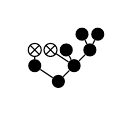
\begin{tikzpicture}[scale=.13333]
          \node[circle, scale=0.5, fill] (tid0) at (4.5,1.5){};
          \node[circle, scale=0.5, fill] (tid2) at (2.25,3){};
          \node[circle, scale=0.5, fill, task_scheduled] (tid4) at (2.25,4.5){};
          \draw[](tid2) -- (tid4);
          \node[circle, scale=0.5, fill] (tid3) at (6,3){};
          \node[circle, scale=0.5, fill, task_scheduled] (tid5) at (3.75,4.5){};
          \node[circle, scale=0.5, fill] (tid6) at (5.25,4.5){};
          \node[circle, scale=0.5, fill] (tid7) at (7.5,4.5){};
          \node[circle, scale=0.5, fill] (tid8) at (6.75,6){};
          \node[circle, scale=0.5, fill] (tid9) at (8.25,6){};
          \draw[](tid7) -- (tid8);
          \draw[](tid7) -- (tid9);
          \draw[](tid3) -- (tid5);
          \draw[](tid3) -- (tid6);
          \draw[](tid3) -- (tid7);
          \draw[](tid0) -- (tid2);
          \draw[](tid0) -- (tid3);
        \end{tikzpicture}
        \nodepart{second}
        5.8906
      }
      ;
      \& 
      \\
    };
  \end{scope}
  \draw (sn0x17d67b0.south) -- (sn0x17d6160.north);
  \draw (sn0x17d67b0.south) -- (sn0x17d55b0.north);
  \draw (sn0x17d67b0.south) -- (sn0x17d2f50.north);
  \draw (sn0x17d67b0.south) -- (sn0x17d5380.north);
  \draw (sn0x17d67b0.south) -- (sn0x17d3a00.north);
  \draw[decorate, decoration=brace] (sn0x17d3a00.north) ++ (0,14) --node [right]{Exp. $\frac{1}{2}$} ++ (0,-13); 
\end{tikzpicture} % successors
    \end{center}
  }
  \only<5>{
    \begin{center}
      \renewcommand{\leveltopI}{-25cm + \leveltop}
\renewcommand{\leveltopII}{-25cm + \leveltopI}
\renewcommand{\leveltopIII}{-16cm + \leveltopII}
\renewcommand{\leveltopIIII}{-12cm + \leveltopIII}
\renewcommand{\leveltopIIIII}{-12cm + \leveltopIIII}
\renewcommand{\leveltopIIIIII}{-12cm + \leveltopIIIII}
\renewcommand{\leveltopIIIIIII}{-12cm + \leveltopIIIIII}
\renewcommand{\leveltopIIIIIIII}{-12cm + \leveltopIIIIIII}
\renewcommand{\leveltopIIIIIIIII}{-12cm + \leveltopIIIIIIII}
\renewcommand{\leveltopIIIIIIIIII}{-12cm + \leveltopIIIIIIIII}
\renewcommand{\leveltopIIIIIIIIIII}{-12cm + \leveltopIIIIIIIIII}
\begin{tikzpicture}[scale=.13333, anchor=south]
  % legende
  %\filldraw[dashed,fill=gray!10!white] (-20, -30) rectangle +(36.5, 12);
  % \draw[dashed] (-30, -13) -- +(60, 0);
  % \draw[dashed] (-30, -24) -- +(60, 0);
  % \node at (10, -21) {Intermediate snapshots};
  \begin{scope}[yshift=\leveltopI cm]
    \matrix (line1)[column sep=0.5cm, ampersand replacement=\&] {
      \node[draw=black, rectangle split,  rectangle split parts=3] (sn0x17d67b0){
        \begin{tikzpicture}[scale=.13333]
          \node[circle, scale=0.5, fill] (tid0) at (4.5,1.5){};
          \node[circle, scale=0.5, fill] (tid2) at (2.25,3){};
          \node[circle, scale=0.5, fill, task_scheduled] (tid4) at (2.25,4.5){};
          \draw[](tid2) -- (tid4);
          \node[circle, scale=0.5, fill] (tid3) at (6,3){};
          \node[circle, scale=0.5, fill] (tid5) at (3.75,4.5){};
          \node[circle, scale=0.5, fill] (tid6) at (5.25,4.5){};
          \node[circle, scale=0.5, fill] (tid7) at (7.5,4.5){};
          \node[circle, scale=0.5, fill] (tid8) at (6.75,6){};
          \node[circle, scale=0.5, fill] (tid9) at (8.25,6){};
          \node[circle, scale=0.5, fill, task_scheduled] (tid10) at (8.25,7.5){};
          \draw[](tid9) -- (tid10);
          \draw[](tid7) -- (tid8);
          \draw[](tid7) -- (tid9);
          \draw[](tid3) -- (tid5);
          \draw[](tid3) -- (tid6);
          \draw[](tid3) -- (tid7);
          \draw[](tid0) -- (tid2);
          \draw[](tid0) -- (tid3);
        \end{tikzpicture}
        \nodepart{second}
        6.43745
        \nodepart{third}
        \footnotesize{10\ 40\ 20\ 10\ 20}
      }
      ;
      \& 
      \\
    };
  \end{scope}
  \begin{scope}[yshift=\leveltopII cm]
    \matrix (line2)[column sep=.5cm, ampersand replacement=\&] {
      \node[draw=black, rectangle split,  rectangle split parts=2] (sn0x17d55b0){
        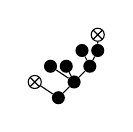
\begin{tikzpicture}[scale=.13333]
          \node[circle, scale=0.5, fill] (tid0) at (4.5,1.5){};
          \node[circle, scale=0.5, fill, task_scheduled] (tid2) at (2.25,3){};
          \node[circle, scale=0.5, fill] (tid3) at (6,3){};
          \node[circle, scale=0.5, fill] (tid5) at (3.75,4.5){};
          \node[circle, scale=0.5, fill] (tid6) at (5.25,4.5){};
          \node[circle, scale=0.5, fill] (tid7) at (7.5,4.5){};
          \node[circle, scale=0.5, fill] (tid8) at (6.75,6){};
          \node[circle, scale=0.5, fill] (tid9) at (8.25,6){};
          \node[circle, scale=0.5, fill, task_scheduled] (tid10) at (8.25,7.5){};
          \draw[](tid9) -- (tid10);
          \draw[](tid7) -- (tid8);
          \draw[](tid7) -- (tid9);
          \draw[](tid3) -- (tid5);
          \draw[](tid3) -- (tid6);
          \draw[](tid3) -- (tid7);
          \draw[](tid0) -- (tid2);
          \draw[](tid0) -- (tid3);
        \end{tikzpicture}
        \nodepart{second}
        6.1640
      }
      ;
      \& 
      \node[draw=black, rectangle split,  rectangle split parts=2] (sn0x17d6160){
        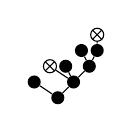
\begin{tikzpicture}[scale=.13333]
          \node[circle, scale=0.5, fill] (tid0) at (4.5,1.5){};
          \node[circle, scale=0.5, fill] (tid2) at (2.25,3){};
          \node[circle, scale=0.5, fill] (tid3) at (6,3){};
          \node[circle, scale=0.5, fill, task_scheduled] (tid5) at (3.75,4.5){};
          \node[circle, scale=0.5, fill] (tid6) at (5.25,4.5){};
          \node[circle, scale=0.5, fill] (tid7) at (7.5,4.5){};
          \node[circle, scale=0.5, fill] (tid8) at (6.75,6){};
          \node[circle, scale=0.5, fill] (tid9) at (8.25,6){};
          \node[circle, scale=0.5, fill, task_scheduled] (tid10) at (8.25,7.5){};
          \draw[](tid9) -- (tid10);
          \draw[](tid7) -- (tid8);
          \draw[](tid7) -- (tid9);
          \draw[](tid3) -- (tid5);
          \draw[](tid3) -- (tid6);
          \draw[](tid3) -- (tid7);
          \draw[](tid0) -- (tid2);
          \draw[](tid0) -- (tid3);
        \end{tikzpicture}
        \nodepart{second}
        5.9921
      }
      ;
      \& 
      \node[draw=black, rectangle split,  rectangle split parts=2] (sn0x17d5380){
        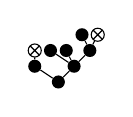
\begin{tikzpicture}[scale=.13333]
          \node[circle, scale=0.5, fill] (tid0) at (4.5,1.5){};
          \node[circle, scale=0.5, fill] (tid2) at (2.25,3){};
          \node[circle, scale=0.5, fill, task_scheduled] (tid4) at (2.25,4.5){};
          \draw[](tid2) -- (tid4);
          \node[circle, scale=0.5, fill] (tid3) at (6,3){};
          \node[circle, scale=0.5, fill] (tid5) at (3.75,4.5){};
          \node[circle, scale=0.5, fill] (tid6) at (5.25,4.5){};
          \node[circle, scale=0.5, fill] (tid7) at (7.5,4.5){};
          \node[circle, scale=0.5, fill] (tid8) at (6.75,6){};
          \node[circle, scale=0.5, fill, task_scheduled] (tid9) at (8.25,6){};
          \draw[](tid7) -- (tid8);
          \draw[](tid7) -- (tid9);
          \draw[](tid3) -- (tid5);
          \draw[](tid3) -- (tid6);
          \draw[](tid3) -- (tid7);
          \draw[](tid0) -- (tid2);
          \draw[](tid0) -- (tid3);
        \end{tikzpicture}
        \nodepart{second}
        5.8203
      }
      ;
      \& 
      \node[draw=black, rectangle split,  rectangle split parts=2] (sn0x17d2f50){
        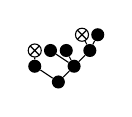
\begin{tikzpicture}[scale=.13333]
          \node[circle, scale=0.5, fill] (tid0) at (4.5,1.5){};
          \node[circle, scale=0.5, fill] (tid2) at (2.25,3){};
          \node[circle, scale=0.5, fill, task_scheduled] (tid4) at (2.25,4.5){};
          \draw[](tid2) -- (tid4);
          \node[circle, scale=0.5, fill] (tid3) at (6,3){};
          \node[circle, scale=0.5, fill] (tid5) at (3.75,4.5){};
          \node[circle, scale=0.5, fill] (tid6) at (5.25,4.5){};
          \node[circle, scale=0.5, fill] (tid7) at (7.5,4.5){};
          \node[circle, scale=0.5, fill, task_scheduled] (tid8) at (6.75,6){};
          \node[circle, scale=0.5, fill] (tid9) at (8.25,6){};
          \draw[](tid7) -- (tid8);
          \draw[](tid7) -- (tid9);
          \draw[](tid3) -- (tid5);
          \draw[](tid3) -- (tid6);
          \draw[](tid3) -- (tid7);
          \draw[](tid0) -- (tid2);
          \draw[](tid0) -- (tid3);
        \end{tikzpicture}
        \nodepart{second}
        5.8203
      }
      ;
      \& 
      \node[draw=black, rectangle split,  rectangle split parts=2] (sn0x17d3a00){
        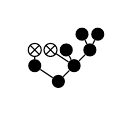
\begin{tikzpicture}[scale=.13333]
          \node[circle, scale=0.5, fill] (tid0) at (4.5,1.5){};
          \node[circle, scale=0.5, fill] (tid2) at (2.25,3){};
          \node[circle, scale=0.5, fill, task_scheduled] (tid4) at (2.25,4.5){};
          \draw[](tid2) -- (tid4);
          \node[circle, scale=0.5, fill] (tid3) at (6,3){};
          \node[circle, scale=0.5, fill, task_scheduled] (tid5) at (3.75,4.5){};
          \node[circle, scale=0.5, fill] (tid6) at (5.25,4.5){};
          \node[circle, scale=0.5, fill] (tid7) at (7.5,4.5){};
          \node[circle, scale=0.5, fill] (tid8) at (6.75,6){};
          \node[circle, scale=0.5, fill] (tid9) at (8.25,6){};
          \draw[](tid7) -- (tid8);
          \draw[](tid7) -- (tid9);
          \draw[](tid3) -- (tid5);
          \draw[](tid3) -- (tid6);
          \draw[](tid3) -- (tid7);
          \draw[](tid0) -- (tid2);
          \draw[](tid0) -- (tid3);
        \end{tikzpicture}
        \nodepart{second}
        5.8906
      }
      ;
      \& 
      \\
    };
  \end{scope}
  \draw (sn0x17d67b0.south) -- (sn0x17d6160.north);
  \draw (sn0x17d67b0.south) -- (sn0x17d55b0.north);
  \draw (sn0x17d67b0.south) -- (sn0x17d2f50.north);
  \draw (sn0x17d67b0.south) -- (sn0x17d5380.north);
  \draw (sn0x17d67b0.south) -- (sn0x17d3a00.north);
\end{tikzpicture} % complete
    \end{center}
  }
  \only<4->{
  \begin{equation*}
    \frac{1}{2}
    + 0.1 \cdot 6.1640
    + 0.4 \cdot 5.9921
    + 0.2 \cdot 5.8203
    + \dots
    % + 0.1 \cdot 5.8203
    % + 0.2 \cdot 5.8906
    = 6.43745
  \end{equation*}
  }
\end{frame}

\begin{frame}
  \frametitle{Equivalent snapshots}
  These two snapshots describe the same:
  \begin{center}
    \begin{tikzpicture}[scale=.2, anchor=south]
\begin{scope}[yshift=\leveltopI cm]
\matrix (line1)[column sep=1cm] {
\node[rectangle split,  rectangle split parts=1] (sn0x8952028){
\begin{tikzpicture}[scale=.2]
\node[circle, scale=0.75, fill] (tid0) at (5.25,1.5){};
\node[circle, scale=0.75, fill] (tid1) at (2.25,3){};
\node[circle, scale=0.75, fill] (tid3) at (1.5,4.5){};
\node[circle, scale=0.75, fill, task_scheduled] (tid8) at (0.75,6){};
\node[circle, scale=0.75, fill, task_scheduled] (tid9) at (2.25,6){};
\draw[](tid3) -- (tid8);
\draw[](tid3) -- (tid9);
\node[circle, scale=0.75, fill] (tid4) at (3.75,4.5){};
\draw[](tid1) -- (tid3);
\draw[](tid1) -- (tid4);
\node[circle, scale=0.75, fill] (tid2) at (7.5,3){};
\node[circle, scale=0.75, fill] (tid5) at (6,4.5){};
\node[circle, scale=0.75, fill] (tid10) at (5.25,6){};
\node[circle, scale=0.75, fill] (tid11) at (6.75,6){};
\draw[](tid5) -- (tid10);
\draw[](tid5) -- (tid11);
\node[circle, scale=0.75, fill] (tid6) at (8.25,4.5){};
\node[circle, scale=0.75, fill, task_scheduled] (tid12) at (8.25,6){};
\draw[](tid6) -- (tid12);
\node[circle, scale=0.75, fill] (tid7) at (9.75,4.5){};
\draw[](tid2) -- (tid5);
\draw[](tid2) -- (tid6);
\draw[](tid2) -- (tid7);
\draw[](tid0) -- (tid1);
\draw[](tid0) -- (tid2);
\end{tikzpicture}
};
\\
};
\end{scope}
\end{tikzpicture}
%%% Local Variables:
%%% TeX-master: "thesis/thesis.tex"
%%% End: 

    \begin{tikzpicture}[scale=.2, anchor=south]
\begin{scope}[yshift=\leveltopI cm]
\matrix (line1)[column sep=1cm] {
\node[rectangle split,  rectangle split parts=1] (sn0x9ef9630){
\begin{tikzpicture}[scale=.2]
\node[circle, scale=0.75, fill] (tid0) at (5.25,1.5){};
\node[circle, scale=0.75, fill] (tid1) at (3,3){};
\node[circle, scale=0.75, fill] (tid3) at (0.75,4.5){};
\node[circle, scale=0.75, fill] (tid4) at (2.25,4.5){};
\node[circle, scale=0.75, fill, task_scheduled] (tid8) at (2.25,6){};
\draw[](tid4) -- (tid8);
\node[circle, scale=0.75, fill] (tid5) at (4.5,4.5){};
\node[circle, scale=0.75, fill] (tid9) at (3.75,6){};
\node[circle, scale=0.75, fill] (tid10) at (5.25,6){};
\draw[](tid5) -- (tid9);
\draw[](tid5) -- (tid10);
\draw[](tid1) -- (tid3);
\draw[](tid1) -- (tid4);
\draw[](tid1) -- (tid5);
\node[circle, scale=0.75, fill] (tid2) at (8.25,3){};
\node[circle, scale=0.75, fill] (tid6) at (6.75,4.5){};
\node[circle, scale=0.75, fill] (tid7) at (9,4.5){};
\node[circle, scale=0.75, fill, task_scheduled] (tid11) at (8.25,6){};
\node[circle, scale=0.75, fill, task_scheduled] (tid12) at (9.75,6){};
\draw[](tid7) -- (tid11);
\draw[](tid7) -- (tid12);
\draw[](tid2) -- (tid6);
\draw[](tid2) -- (tid7);
\draw[](tid0) -- (tid1);
\draw[](tid0) -- (tid2);
\end{tikzpicture}
};
\\
};
\end{scope}
\end{tikzpicture}
%%% Local Variables:
%%% TeX-master: "thesis/thesis.tex"
%%% End: 

  \end{center}
  \begin{block}{Equivalent snapshots}
    \begin{itemize}
    \item Isomorphic intrees
    \item Scheduled tasks are mapped onto each other
    \item Equivalent snapshots excluded/re-used if they result from the same finishing task
    \item \emph{Canonical} snapshots constructable in $O(n)$
    \end{itemize}
  \end{block}
\end{frame}

\begin{frame}
  \frametitle{Equivalent snapshots --- example}
  \begin{center}
    \only<1>{
      \renewcommand{\leveltopI}{-10cm + \leveltop}
\renewcommand{\leveltopII}{-10cm + \leveltopI}
\begin{tikzpicture}[scale=.2, anchor=south]
  \node[text width=4cm](info) at (14,-10){Each transition shown has a probability of $\frac{1}{6}$.};
  \draw[->, dashed] (info) ..controls+(0,-2)and+(+2,0).. +(-5,-5);
  \draw[->, dashed] (info) ..controls+(0,-2)and+(+2,0).. +(-11,-5);
  \tikzstyle{task_scheduled}=[fill=white, draw]
  \begin{scope}[yshift=\leveltopI cm]
    \matrix (line1)[column sep=0.25cm] {
      \node[draw=black, rectangle split,  rectangle split parts=1] (sn0x9bc9928){
        \begin{tikzpicture}[scale=.2]
          \node[circle, scale=0.4286, fill=white!80!black, draw=black] (tid0) at (3.75,1.5){\scriptsize{0}};
          \node[circle, scale=0.4286, fill=white!80!black, draw=black] (tid1) at (1.5,3){\scriptsize{1}};
          \node[circle, scale=0.4286, fill, task_scheduled] (tid4) at (0.75,4.5){\scriptsize{4}};
          \node[circle, scale=0.4286, fill, task_scheduled] (tid6) at (2.25,4.5){\scriptsize{6}};
          \draw[](tid1) -- (tid4);
          \draw[](tid1) -- (tid6);
          \node[circle, scale=0.4286, fill, task_scheduled] (tid2) at (3.75,3){\scriptsize{2}};
          \node[circle, scale=0.4286, fill=white!80!black, draw=black] (tid3) at (5.25,3){\scriptsize{3}};
          \node[circle, scale=0.4286, fill=white!80!black, draw=black] (tid5) at (6.75,3){\scriptsize{5}};
          \draw[](tid0) -- (tid1);
          \draw[](tid0) -- (tid2);
          \draw[](tid0) -- (tid3);
          \draw[](tid0) -- (tid5);
        \end{tikzpicture}
      };
      & 
      \\
    };
  \end{scope}
  \begin{scope}[yshift=\leveltopII cm]
    \matrix (line2)[column sep=0.25cm] {
      \node[draw=black, rectangle split,  rectangle split parts=1] (sn0x9bcb370){
        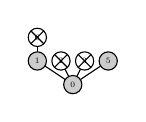
\begin{tikzpicture}[scale=.2]
          \node[circle, scale=0.4286, fill=white!80!black, draw=black] (tid0) at (3,1.5){\scriptsize{0}};
          \node[circle, scale=0.4286, fill=white!80!black, draw=black] (tid1) at (0.75,3){\scriptsize{1}};
          \node[circle, scale=0.4286, fill, task_scheduled] (tid6) at (0.75,4.5){\scriptsize{6}};
          \draw[](tid1) -- (tid6);
          \node[circle, scale=0.4286, fill, task_scheduled] (tid2) at (2.25,3){\scriptsize{2}};
          \node[circle, scale=0.4286, fill, task_scheduled] (tid3) at (3.75,3){\scriptsize{3}};
          \node[circle, scale=0.4286, fill=white!80!black, draw=black] (tid5) at (5.25,3){\scriptsize{5}};
          \draw[](tid0) -- (tid1);
          \draw[](tid0) -- (tid2);
          \draw[](tid0) -- (tid3);
          \draw[](tid0) -- (tid5);
        \end{tikzpicture}
      };
      & 
      \node[draw=black, rectangle split,  rectangle split parts=1] (sn0x9bd1828){
        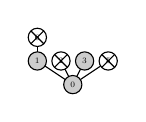
\begin{tikzpicture}[scale=.2]
          \node[circle, scale=0.4286, fill=white!80!black, draw=black] (tid0) at (3,1.5){\scriptsize{0}};
          \node[circle, scale=0.4286, fill=white!80!black, draw=black] (tid1) at (0.75,3){\scriptsize{1}};
          \node[circle, scale=0.4286, fill, task_scheduled] (tid6) at (0.75,4.5){\scriptsize{6}};
          \draw[](tid1) -- (tid6);
          \node[circle, scale=0.4286, fill, task_scheduled] (tid2) at (2.25,3){\scriptsize{2}};
          \node[circle, scale=0.4286, fill=white!80!black, draw=black] (tid3) at (3.75,3){\scriptsize{3}};
          \node[circle, scale=0.4286, fill, task_scheduled] (tid5) at (5.25,3){\scriptsize{5}};
          \draw[](tid0) -- (tid1);
          \draw[](tid0) -- (tid2);
          \draw[](tid0) -- (tid3);
          \draw[](tid0) -- (tid5);
        \end{tikzpicture}
      };
      & 
      \node[draw=black, rectangle split,  rectangle split parts=1] (sn0x9bd0f28){
        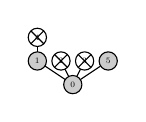
\begin{tikzpicture}[scale=.2]
          \node[circle, scale=0.4286, fill=white!80!black, draw=black] (tid0) at (3,1.5){\scriptsize{0}};
          \node[circle, scale=0.4286, fill=white!80!black, draw=black] (tid1) at (0.75,3){\scriptsize{1}};
          \node[circle, scale=0.4286, fill, task_scheduled] (tid4) at (0.75,4.5){\scriptsize{4}};
          \draw[](tid1) -- (tid4);
          \node[circle, scale=0.4286, fill, task_scheduled] (tid2) at (2.25,3){\scriptsize{2}};
          \node[circle, scale=0.4286, fill, task_scheduled] (tid3) at (3.75,3){\scriptsize{3}};
          \node[circle, scale=0.4286, fill=white!80!black, draw=black] (tid5) at (5.25,3){\scriptsize{5}};
          \draw[](tid0) -- (tid1);
          \draw[](tid0) -- (tid2);
          \draw[](tid0) -- (tid3);
          \draw[](tid0) -- (tid5);
        \end{tikzpicture}
      };
      & 
      \node[draw=black, rectangle split,  rectangle split parts=1] (sn0x9bd2140){
        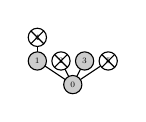
\begin{tikzpicture}[scale=.2]
          \node[circle, scale=0.4286, fill=white!80!black, draw=black] (tid0) at (3,1.5){\scriptsize{0}};
          \node[circle, scale=0.4286, fill=white!80!black, draw=black] (tid1) at (0.75,3){\scriptsize{1}};
          \node[circle, scale=0.4286, fill, task_scheduled] (tid4) at (0.75,4.5){\scriptsize{4}};
          \draw[](tid1) -- (tid4);
          \node[circle, scale=0.4286, fill, task_scheduled] (tid2) at (2.25,3){\scriptsize{2}};
          \node[circle, scale=0.4286, fill=white!80!black, draw=black] (tid3) at (3.75,3){\scriptsize{3}};
          \node[circle, scale=0.4286, fill, task_scheduled] (tid5) at (5.25,3){\scriptsize{5}};
          \draw[](tid0) -- (tid1);
          \draw[](tid0) -- (tid2);
          \draw[](tid0) -- (tid3);
          \draw[](tid0) -- (tid5);
        \end{tikzpicture}
      };
      & 
      \node[draw=black, rectangle split,  rectangle split parts=1] (sn0x9bc7440){
        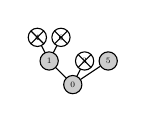
\begin{tikzpicture}[scale=.2]
          \node[circle, scale=0.4286, fill=white!80!black, draw=black] (tid0) at (3,1.5){\scriptsize{0}};
          \node[circle, scale=0.4286, fill=white!80!black, draw=black] (tid1) at (1.5,3){\scriptsize{1}};
          \node[circle, scale=0.4286, fill, task_scheduled] (tid4) at (0.75,4.5){\scriptsize{4}};
          \node[circle, scale=0.4286, fill, task_scheduled] (tid6) at (2.25,4.5){\scriptsize{6}};
          \draw[](tid1) -- (tid4);
          \draw[](tid1) -- (tid6);
          \node[circle, scale=0.4286, fill, task_scheduled] (tid3) at (3.75,3){\scriptsize{3}};
          \node[circle, scale=0.4286, fill=white!80!black, draw=black] (tid5) at (5.25,3){\scriptsize{5}};
          \draw[](tid0) -- (tid1);
          \draw[](tid0) -- (tid3);
          \draw[](tid0) -- (tid5);
        \end{tikzpicture}
      };
      & 
      \node[draw=black, rectangle split,  rectangle split parts=1] (sn0x9bd1530){
        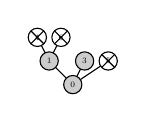
\begin{tikzpicture}[scale=.2]
          \node[circle, scale=0.4286, fill=white!80!black, draw=black] (tid0) at (3,1.5){\scriptsize{0}};
          \node[circle, scale=0.4286, fill=white!80!black, draw=black] (tid1) at (1.5,3){\scriptsize{1}};
          \node[circle, scale=0.4286, fill, task_scheduled] (tid4) at (0.75,4.5){\scriptsize{4}};
          \node[circle, scale=0.4286, fill, task_scheduled] (tid6) at (2.25,4.5){\scriptsize{6}};
          \draw[](tid1) -- (tid4);
          \draw[](tid1) -- (tid6);
          \node[circle, scale=0.4286, fill=white!80!black, draw=black] (tid3) at (3.75,3){\scriptsize{3}};
          \node[circle, scale=0.4286, fill, task_scheduled] (tid5) at (5.25,3){\scriptsize{5}};
          \draw[](tid0) -- (tid1);
          \draw[](tid0) -- (tid3);
          \draw[](tid0) -- (tid5);
        \end{tikzpicture}
      };
      & 
      \\
    };
  \end{scope}
  \draw (sn0x9bc9928.south) -- (sn0x9bc7440.north);
  \draw (sn0x9bc9928.south) -- (sn0x9bd1530.north);
  \draw (sn0x9bc9928.south) -- (sn0x9bcb370.north);
  \draw (sn0x9bc9928.south) -- (sn0x9bd1828.north);
  \draw (sn0x9bc9928.south) -- (sn0x9bd0f28.north);
  \draw (sn0x9bc9928.south) -- (sn0x9bd2140.north);
  \begin{scope}[yshift=-3cm]
    \draw[decorate,decoration={brace,mirror}] (-25.5,-17)
    --node[below, yshift=-.1cm]{Task 4 finished first} +(16.1,0);
    \draw[decorate,decoration={brace,mirror}] (-8.7,-17)
    --node[below, yshift=-.1cm]{Task 6 finished first} +(16.1,0);
    \draw[decorate,decoration={brace,mirror}] (8.2,-17)
    --node[below, yshift=-.1cm]{Task 2 finished first} +(16.1,0);
    % equivalences
    \draw[decorate,decoration={brace,mirror}] (-25.5,-22)
    --node[below, yshift=-.1cm]{4 equivalent snapshots} +(32.6,0);
    \draw[decorate,decoration={brace,mirror}] (8.2,-22)
    --node[below, yshift=-.1cm]{2 equivalent snapshots} +(16.1,0);
  \end{scope}
\end{tikzpicture}

    }
    \only<2>{
      \renewcommand{\leveltopI}{-10cm + \leveltop}
\renewcommand{\leveltopII}{-10cm + \leveltopI}
\begin{tikzpicture}[scale=.2, anchor=south]
  \begin{scope}[yshift=\leveltopI cm]
    \matrix (line1)[column sep=0.25cm] {
      \node[draw=black, rectangle split,  rectangle split parts=1] (sn0x9bc9928){
        \begin{tikzpicture}[scale=.2]
          \node[circle, scale=0.75, fill, draw=black] (tid0) at (3.75,1.5){};
          \node[circle, scale=0.75, fill, draw=black] (tid1) at (1.5,3){};
          \node[circle, scale=0.75, fill, task_scheduled] (tid4) at (0.75,4.5){};
          \node[circle, scale=0.75, fill, task_scheduled] (tid6) at (2.25,4.5){};
          \draw[](tid1) -- (tid4);
          \draw[](tid1) -- (tid6);
          \node[circle, scale=0.75, fill, task_scheduled] (tid2) at (3.75,3){};
          \node[circle, scale=0.75, fill, draw=black] (tid3) at (5.25,3){};
          \node[circle, scale=0.75, fill, draw=black] (tid5) at (6.75,3){};
          \draw[](tid0) -- (tid1);
          \draw[](tid0) -- (tid2);
          \draw[](tid0) -- (tid3);
          \draw[](tid0) -- (tid5);
        \end{tikzpicture}
      };
      & 
      \\
    };
  \end{scope}
  \begin{scope}[yshift=\leveltopII cm]
    \matrix (line2)[column sep=0.25cm] {
      \node[draw=black, rectangle split,  rectangle split parts=1] (sn0x9bd2140){
        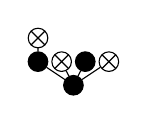
\begin{tikzpicture}[scale=.2]
          \node[circle, scale=0.75, fill, draw=black] (tid0) at (3,1.5){};
          \node[circle, scale=0.75, fill, draw=black] (tid1) at (0.75,3){};
          \node[circle, scale=0.75, fill, task_scheduled] (tid4) at (0.75,4.5){};
          \draw[](tid1) -- (tid4);
          \node[circle, scale=0.75, fill, task_scheduled] (tid2) at (2.25,3){};
          \node[circle, scale=0.75, fill, draw=black] (tid3) at (3.75,3){};
          \node[circle, scale=0.75, fill, task_scheduled] (tid5) at (5.25,3){};
          \draw[](tid0) -- (tid1);
          \draw[](tid0) -- (tid2);
          \draw[](tid0) -- (tid3);
          \draw[](tid0) -- (tid5);
        \end{tikzpicture}
      };
      & 
      \node[draw=black, rectangle split,  rectangle split parts=1] (sn0x9bc7440){
        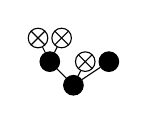
\begin{tikzpicture}[scale=.2]
          \node[circle, scale=0.75, fill, draw=black] (tid0) at (3,1.5){};
          \node[circle, scale=0.75, fill, draw=black] (tid1) at (1.5,3){};
          \node[circle, scale=0.75, fill, task_scheduled] (tid4) at (0.75,4.5){};
          \node[circle, scale=0.75, fill, task_scheduled] (tid6) at (2.25,4.5){};
          \draw[](tid1) -- (tid4);
          \draw[](tid1) -- (tid6);
          \node[circle, scale=0.75, fill, task_scheduled] (tid3) at (3.75,3){};
          \node[circle, scale=0.75, fill, draw=black] (tid5) at (5.25,3){};
          \draw[](tid0) -- (tid1);
          \draw[](tid0) -- (tid3);
          \draw[](tid0) -- (tid5);
        \end{tikzpicture}
      };
      & 
      \\
    };
  \end{scope}
  \draw[] (sn0x9bc9928.south) --node[right,xshift=.1cm]{$\frac{2}{6}$} (sn0x9bc7440.north);
  \draw[] (sn0x9bc9928.south) --node[left,xshift=-.1cm]{$\frac{4}{6}$} (sn0x9bd2140.north);
\end{tikzpicture}

    }
  \end{center}
\end{frame}

\section{Two processors}

\subsection{Optimal solution}

\begin{frame}
  \frametitle{Two processors --- optimal solution}
  \begin{columns}
    \begin{column}{0.6\textwidth}
      \begin{block}{Known results (Chandy, Reynolds 1975)}
        \begin{itemize}
        \item Highest-level-first (HLF) optimal for two processors
        \item Profile (number of tasks per level) completely determines run time
        \item Reduce computation of expected run time to profiles
        \end{itemize}
      \end{block}
    \end{column}
    \begin{column}{.4\textwidth}
      \renewcommand{\leveltopI}{-10cm + \leveltop}
\renewcommand{\leveltopII}{-10cm + \leveltopI}
\renewcommand{\leveltopIII}{-10cm + \leveltopII}
\renewcommand{\leveltopIIII}{-10cm + \leveltopIII}
\renewcommand{\leveltopIIIII}{-10cm + \leveltopIIII}
\renewcommand{\leveltopIIIIII}{-10cm + \leveltopIIIII}
\renewcommand{\leveltopIIIIIII}{-10cm + \leveltopIIIIII}
\renewcommand{\leveltopIIIIIIII}{-10cm + \leveltopIIIIIII}
\begin{tikzpicture}[scale=.2, anchor=south]
\begin{scope}[yshift=\leveltopI cm]
\matrix (line1)[column sep=1cm] {
\node[draw=black, rectangle split,  rectangle split parts=2] (sn0x94980e8){
\begin{tikzpicture}[scale=.2]
\node[circle, scale=0.75, fill] (tid0) at (3.75,1.5){};
\node[circle, scale=0.75, fill] (tid1) at (0.75,3){};
\node[circle, scale=0.75, fill] (tid2) at (3.75,3){};
\node[circle, scale=0.75, fill, task_scheduled] (tid4) at (2.25,4.5){};
\node[circle, scale=0.75, fill] (tid5) at (3.75,4.5){};
\node[circle, scale=0.75, fill] (tid6) at (5.25,4.5){};
\draw[](tid2) -- (tid4);
\draw[](tid2) -- (tid5);
\draw[](tid2) -- (tid6);
\node[circle, scale=0.75, fill] (tid3) at (6.75,3){};
\node[circle, scale=0.75, fill, task_scheduled] (tid7) at (6.75,4.5){};
\draw[](tid3) -- (tid7);
\draw[](tid0) -- (tid1);
\draw[](tid0) -- (tid2);
\draw[](tid0) -- (tid3);
\end{tikzpicture}
\nodepart{two}
\footnotesize{5.125}
};
\\
};
\end{scope}
\begin{scope}[yshift=\leveltopII cm]
\matrix (line2)[column sep=1cm] {
\node[draw=black, rectangle split,  rectangle split parts=2] (sn0x9497e38){
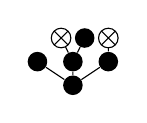
\begin{tikzpicture}[scale=.2]
\node[circle, scale=0.75, fill] (tid0) at (3,1.5){};
\node[circle, scale=0.75, fill] (tid1) at (0.75,3){};
\node[circle, scale=0.75, fill] (tid2) at (3,3){};
\node[circle, scale=0.75, fill, task_scheduled] (tid4) at (2.25,4.5){};
\node[circle, scale=0.75, fill] (tid5) at (3.75,4.5){};
\draw[](tid2) -- (tid4);
\draw[](tid2) -- (tid5);
\node[circle, scale=0.75, fill] (tid3) at (5.25,3){};
\node[circle, scale=0.75, fill, task_scheduled] (tid6) at (5.25,4.5){};
\draw[](tid3) -- (tid6);
\draw[](tid0) -- (tid1);
\draw[](tid0) -- (tid2);
\draw[](tid0) -- (tid3);
\end{tikzpicture}
\nodepart{two}
\footnotesize{4.625}
};
 & 
\node[draw=black, rectangle split,  rectangle split parts=2] (sn0x9498010){
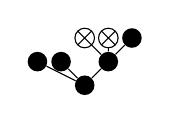
\begin{tikzpicture}[scale=.2]
\node[circle, scale=0.75, fill] (tid0) at (3.75,1.5){};
\node[circle, scale=0.75, fill] (tid1) at (0.75,3){};
\node[circle, scale=0.75, fill] (tid2) at (2.25,3){};
\node[circle, scale=0.75, fill] (tid3) at (5.25,3){};
\node[circle, scale=0.75, fill, task_scheduled] (tid4) at (3.75,4.5){};
\node[circle, scale=0.75, fill, task_scheduled] (tid5) at (5.25,4.5){};
\node[circle, scale=0.75, fill] (tid6) at (6.75,4.5){};
\draw[](tid3) -- (tid4);
\draw[](tid3) -- (tid5);
\draw[](tid3) -- (tid6);
\draw[](tid0) -- (tid1);
\draw[](tid0) -- (tid2);
\draw[](tid0) -- (tid3);
\end{tikzpicture}
\nodepart{two}
\footnotesize{4.625}
};
\\
};
\end{scope}
\begin{scope}[yshift=\leveltopIII cm]
\matrix (line3)[column sep=1cm] {
\node[draw=black, rectangle split,  rectangle split parts=2] (sn0x9497bb0){
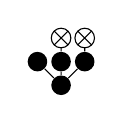
\begin{tikzpicture}[scale=.2]
\node[circle, scale=0.75, fill] (tid0) at (2.25,1.5){};
\node[circle, scale=0.75, fill] (tid1) at (0.75,3){};
\node[circle, scale=0.75, fill] (tid2) at (2.25,3){};
\node[circle, scale=0.75, fill, task_scheduled] (tid4) at (2.25,4.5){};
\draw[](tid2) -- (tid4);
\node[circle, scale=0.75, fill] (tid3) at (3.75,3){};
\node[circle, scale=0.75, fill, task_scheduled] (tid5) at (3.75,4.5){};
\draw[](tid3) -- (tid5);
\draw[](tid0) -- (tid1);
\draw[](tid0) -- (tid2);
\draw[](tid0) -- (tid3);
\end{tikzpicture}
\nodepart{two}
\footnotesize{4.125}
};
 & 
\node[draw=black, rectangle split,  rectangle split parts=2] (sn0x9497d60){
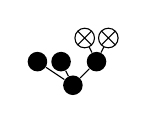
\begin{tikzpicture}[scale=.2]
\node[circle, scale=0.75, fill] (tid0) at (3,1.5){};
\node[circle, scale=0.75, fill] (tid1) at (0.75,3){};
\node[circle, scale=0.75, fill] (tid2) at (2.25,3){};
\node[circle, scale=0.75, fill] (tid3) at (4.5,3){};
\node[circle, scale=0.75, fill, task_scheduled] (tid4) at (3.75,4.5){};
\node[circle, scale=0.75, fill, task_scheduled] (tid5) at (5.25,4.5){};
\draw[](tid3) -- (tid4);
\draw[](tid3) -- (tid5);
\draw[](tid0) -- (tid1);
\draw[](tid0) -- (tid2);
\draw[](tid0) -- (tid3);
\end{tikzpicture}
\nodepart{two}
\footnotesize{4.125}
};
\\
};
\end{scope}
\draw (sn0x94980e8.south) -- (sn0x9497e38.north);
\draw (sn0x94980e8.south) -- (sn0x9498010.north);
\draw (sn0x9497e38.south) -- (sn0x9497bb0.north);
\draw (sn0x9497e38.south) -- (sn0x9497d60.north);
\draw (sn0x9498010.south) -- (sn0x9497d60.north);
\end{tikzpicture}
%%% Local Variables:
%%% TeX-master: "thesis/thesis.tex"
%%% End: 

    \end{column}
  \end{columns}
  %   \begin{exampleblock}{Profiles: Intrees with profile $\profile{6,3,1}$ (run time $7.125$):}
  %   % \begin{center}
  %   %   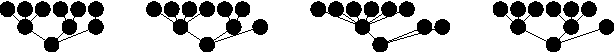
\includegraphics{../thesis/p2/four_profiles_631.pdf}  
  %   % \end{center}
  % \end{exampleblock}
\end{frame}

% \begin{frame}
%   \frametitle{HLF example}
%   \begin{center}
%     \renewcommand{\leveltopI}{-10cm + \leveltop}
\renewcommand{\leveltopII}{-10cm + \leveltopI}
\renewcommand{\leveltopIII}{-10cm + \leveltopII}
\renewcommand{\leveltopIIII}{-10cm + \leveltopIII}
\renewcommand{\leveltopIIIII}{-10cm + \leveltopIIII}
\renewcommand{\leveltopIIIIII}{-10cm + \leveltopIIIII}
\renewcommand{\leveltopIIIIIII}{-10cm + \leveltopIIIIII}
\renewcommand{\leveltopIIIIIIII}{-10cm + \leveltopIIIIIII}
\begin{tikzpicture}[scale=.2, anchor=south]
\begin{scope}[yshift=\leveltopI cm]
\matrix (line1)[column sep=1cm] {
\node[draw=black, rectangle split,  rectangle split parts=2] (sn0x94980e8){
\begin{tikzpicture}[scale=.2]
\node[circle, scale=0.75, fill] (tid0) at (3.75,1.5){};
\node[circle, scale=0.75, fill] (tid1) at (0.75,3){};
\node[circle, scale=0.75, fill] (tid2) at (3.75,3){};
\node[circle, scale=0.75, fill, task_scheduled] (tid4) at (2.25,4.5){};
\node[circle, scale=0.75, fill] (tid5) at (3.75,4.5){};
\node[circle, scale=0.75, fill] (tid6) at (5.25,4.5){};
\draw[](tid2) -- (tid4);
\draw[](tid2) -- (tid5);
\draw[](tid2) -- (tid6);
\node[circle, scale=0.75, fill] (tid3) at (6.75,3){};
\node[circle, scale=0.75, fill, task_scheduled] (tid7) at (6.75,4.5){};
\draw[](tid3) -- (tid7);
\draw[](tid0) -- (tid1);
\draw[](tid0) -- (tid2);
\draw[](tid0) -- (tid3);
\end{tikzpicture}
\nodepart{two}
\footnotesize{5.125}
};
\\
};
\end{scope}
\begin{scope}[yshift=\leveltopII cm]
\matrix (line2)[column sep=1cm] {
\node[draw=black, rectangle split,  rectangle split parts=2] (sn0x9497e38){
\begin{tikzpicture}[scale=.2]
\node[circle, scale=0.75, fill] (tid0) at (3,1.5){};
\node[circle, scale=0.75, fill] (tid1) at (0.75,3){};
\node[circle, scale=0.75, fill] (tid2) at (3,3){};
\node[circle, scale=0.75, fill, task_scheduled] (tid4) at (2.25,4.5){};
\node[circle, scale=0.75, fill] (tid5) at (3.75,4.5){};
\draw[](tid2) -- (tid4);
\draw[](tid2) -- (tid5);
\node[circle, scale=0.75, fill] (tid3) at (5.25,3){};
\node[circle, scale=0.75, fill, task_scheduled] (tid6) at (5.25,4.5){};
\draw[](tid3) -- (tid6);
\draw[](tid0) -- (tid1);
\draw[](tid0) -- (tid2);
\draw[](tid0) -- (tid3);
\end{tikzpicture}
\nodepart{two}
\footnotesize{4.625}
};
 & 
\node[draw=black, rectangle split,  rectangle split parts=2] (sn0x9498010){
\begin{tikzpicture}[scale=.2]
\node[circle, scale=0.75, fill] (tid0) at (3.75,1.5){};
\node[circle, scale=0.75, fill] (tid1) at (0.75,3){};
\node[circle, scale=0.75, fill] (tid2) at (2.25,3){};
\node[circle, scale=0.75, fill] (tid3) at (5.25,3){};
\node[circle, scale=0.75, fill, task_scheduled] (tid4) at (3.75,4.5){};
\node[circle, scale=0.75, fill, task_scheduled] (tid5) at (5.25,4.5){};
\node[circle, scale=0.75, fill] (tid6) at (6.75,4.5){};
\draw[](tid3) -- (tid4);
\draw[](tid3) -- (tid5);
\draw[](tid3) -- (tid6);
\draw[](tid0) -- (tid1);
\draw[](tid0) -- (tid2);
\draw[](tid0) -- (tid3);
\end{tikzpicture}
\nodepart{two}
\footnotesize{4.625}
};
\\
};
\end{scope}
\begin{scope}[yshift=\leveltopIII cm]
\matrix (line3)[column sep=1cm] {
\node[draw=black, rectangle split,  rectangle split parts=2] (sn0x9497bb0){
\begin{tikzpicture}[scale=.2]
\node[circle, scale=0.75, fill] (tid0) at (2.25,1.5){};
\node[circle, scale=0.75, fill] (tid1) at (0.75,3){};
\node[circle, scale=0.75, fill] (tid2) at (2.25,3){};
\node[circle, scale=0.75, fill, task_scheduled] (tid4) at (2.25,4.5){};
\draw[](tid2) -- (tid4);
\node[circle, scale=0.75, fill] (tid3) at (3.75,3){};
\node[circle, scale=0.75, fill, task_scheduled] (tid5) at (3.75,4.5){};
\draw[](tid3) -- (tid5);
\draw[](tid0) -- (tid1);
\draw[](tid0) -- (tid2);
\draw[](tid0) -- (tid3);
\end{tikzpicture}
\nodepart{two}
\footnotesize{4.125}
};
 & 
\node[draw=black, rectangle split,  rectangle split parts=2] (sn0x9497d60){
\begin{tikzpicture}[scale=.2]
\node[circle, scale=0.75, fill] (tid0) at (3,1.5){};
\node[circle, scale=0.75, fill] (tid1) at (0.75,3){};
\node[circle, scale=0.75, fill] (tid2) at (2.25,3){};
\node[circle, scale=0.75, fill] (tid3) at (4.5,3){};
\node[circle, scale=0.75, fill, task_scheduled] (tid4) at (3.75,4.5){};
\node[circle, scale=0.75, fill, task_scheduled] (tid5) at (5.25,4.5){};
\draw[](tid3) -- (tid4);
\draw[](tid3) -- (tid5);
\draw[](tid0) -- (tid1);
\draw[](tid0) -- (tid2);
\draw[](tid0) -- (tid3);
\end{tikzpicture}
\nodepart{two}
\footnotesize{4.125}
};
\\
};
\end{scope}
\draw (sn0x94980e8.south) -- (sn0x9497e38.north);
\draw (sn0x94980e8.south) -- (sn0x9498010.north);
\draw (sn0x9497e38.south) -- (sn0x9497bb0.north);
\draw (sn0x9497e38.south) -- (sn0x9497d60.north);
\draw (sn0x9498010.south) -- (sn0x9497d60.north);
\end{tikzpicture}
%%% Local Variables:
%%% TeX-master: "thesis/thesis.tex"
%%% End: 

%   \end{center}
% \end{frame}

\subsection{Expected run time}

% \begin{frame}
%   \frametitle{Expected run time}
%   \begin{block}{Function $SUC$:}
%     \begin{equation*}
%       SUC(\profile{n_1,\dots,n_r}) = \profile{n_1, n_2, n_3,\dots,n_{j-1},n_j-1,n_{j+1},\dots,n_r} 
%     \end{equation*}
%     such that $j$ is the minimum index such that $n_j>1$.  
%   \end{block}
%   \begin{block}{Optimal (i.e. HLF) expected run time}
%     Let $P=\profile{n_1}\profileconcat P'$. Then
%     \begin{equation*}
%       \E{P} =
%       \begin{cases}
%         r, & \text{ if } P = \profile{\profileones r} \\
%         \frac{1}{2} + \E{\profile{n_1-1}\profileconcat P'} , & \text{ if } n_1\geq 2 \\
%         \frac{1}{2} + \frac{1}{2} \cdot \left( \E{P'} + \E{SUC(P)} \right) ,& \text{ otherwise } 
%       \end{cases}.
%     \end{equation*}
%   \end{block}
% \end{frame}

\begin{frame}
  \frametitle{Expected run time --- two-leaves intrees}
  \begin{theorem}[Maaß 2001]
    Let $l, k\in\naturals$, $a\in\naturals_0$. Intrees with profile $\profile{\profilerepeat{1}{l-k}, \profilerepeat{2}{k}, \profilerepeat{1}{a+1}}$ have expected run time
    \begin{align*}
      & \sum_{i=1}^k \left(\frac{1}{2}\right)^{l+i-1} \cdot \binom{l+i-2}{i-1} \cdot \left( k-i+2 \right) \\
       & + \sum_{j=1}^l \left(\frac{1}{2}\right)^{k+j-1} \cdot \binom{k+j-2}{j-1} \cdot \left( l-j+2 \right) \\
       & + \sum_{i=1}^k \sum_{j=1}^l \left( \frac{1}{2}^{k-i+l-j+1}\cdot\binom{ki+l-j}{l-j} \right) \\
       & + a
      .
    \end{align*}
  \end{theorem}
\end{frame}

\begin{frame}
  \frametitle{Expected run time --- intrees with many 1-levels}
  \begin{theorem}
    Intrees with profile $\profile{n_1,\profileones{j-2},n_j,\profileones{r-j}}$ (for $j\geq 2$) has expected run time
    \begin{equation*}
      \E{\profile{n_1,\profileones{j-2},n_j,\profileones{r-j}}} = 
      r + \frac{A_0(n_1-2)}{2^{n_1-1}} + \frac{A_{j-1}(n_j-2)}{2^{n_j+j-2}},
    \end{equation*}
    where $A_i$ is inductively defined as follows:
    \begin{equation*}
      A_0(n) = (n+1) \cdot 2^n \quad 
      A_{i+1}(n) = \sum_{k=0}^n A_{i}(k)
    \end{equation*}
    \note{Closed forms $A_j$ for fixed $j$ known}
  \end{theorem}
\end{frame}

\subsection{Profile DAG}

\begin{frame}
  \frametitle{Profile DAG}
  \begin{itemize}
  \item Use profiles instead of whole snapshots
  \item Scheduled tasks given implicitly (HLF)
  \item Worst case profile $\profile{ \profileones{ \left\lfloor\frac{n}{2} \right\rfloor - 1}, \left\lceil \frac{n}{2} \right\rceil, 1 }$
  \item Worst case profile DAG size has $\lfloor \frac{n}{2} \rfloor \cdot \lceil \frac{n}{2} \rceil +1$ ``profile snapshots''
  \item Each profile snapshot accounts for less than $n^2$ ``original snapshots''
    
    $\Rightarrow$ Simple proof: At most $O(n^4)$ original snapshots.
  \end{itemize}
\end{frame}

\section{Three processors: strategies}

\subsection{HLF}

\begin{frame}
  \frametitle{HLF may be ambiguous \dots}
  HLF may result in different run times:
  \begin{block}{}
    \begin{columns}
  \begin{column}{.45\textwidth}
    \centering
    \renewcommand{\leveltopI}{-12cm + \leveltop}
    \renewcommand{\leveltopII}{-12cm + \leveltopI}
    \renewcommand{\leveltopIII}{-12cm + \leveltopII}
    \renewcommand{\leveltopIIII}{-15cm + \leveltopIII}
    \renewcommand{\leveltopIIIII}{-15cm + \leveltopIIII}
    \renewcommand{\leveltopIIIIII}{-15cm + \leveltopIIIII}
    \renewcommand{\leveltopIIIIIII}{-15cm + \leveltopIIIIII}
    \begin{tikzpicture}[scale=.2, anchor=south]
      \begin{scope}[yshift=\leveltopI cm]
        \matrix (line1)[column sep=1cm] {
          \node[draw=black, rectangle split,  rectangle split parts=3] (sn0x938eff0){
            \begin{tikzpicture}[scale=.2]
              \node[circle, scale=0.75, fill] (tid0) at (3,1.5){};
              \node[circle, scale=0.75, fill] (tid1) at (2.25,3){};
              \node[circle, scale=0.75, fill, task_scheduled] (tid3) at (0.75,4.5){};
              \node[circle, scale=0.75, fill, task_scheduled] (tid4) at (2.25,4.5){};
              \node[circle, scale=0.75, fill, task_scheduled] (tid5) at (3.75,4.5){};
              \draw[](tid1) -- (tid3);
              \draw[](tid1) -- (tid4);
              \draw[](tid1) -- (tid5);
              \node[circle, scale=0.75, fill] (tid2) at (5.25,3){};
              \node[circle, scale=0.75, fill] (tid6) at (5.25,4.5){};
              \draw[](tid2) -- (tid6);
              \draw[](tid0) -- (tid1);
              \draw[](tid0) -- (tid2);
            \end{tikzpicture}
            \nodepart{two}
            \footnotesize{4.38889}
            \nodepart{three}
            \footnotesize{$100$}
          };
          & 
          \\
        };
      \end{scope}
      \begin{scope}[yshift=\leveltopII cm]
        \matrix (line2)[column sep=1cm] {
          \node[draw=black, rectangle split,  rectangle split parts=3] (sn0x938dbf0){
            \begin{tikzpicture}[scale=.2]
              \node[circle, scale=0.75, fill] (tid0) at (2.25,1.5){};
              \node[circle, scale=0.75, fill] (tid1) at (1.5,3){};
              \node[circle, scale=0.75, fill, task_scheduled] (tid3) at (0.75,4.5){};
              \node[circle, scale=0.75, fill, task_scheduled] (tid4) at (2.25,4.5){};
              \draw[](tid1) -- (tid3);
              \draw[](tid1) -- (tid4);
              \node[circle, scale=0.75, fill] (tid2) at (3.75,3){};
              \node[circle, scale=0.75, fill, task_scheduled] (tid5) at (3.75,4.5){};
              \draw[](tid2) -- (tid5);
              \draw[](tid0) -- (tid1);
              \draw[](tid0) -- (tid2);
            \end{tikzpicture}
            \nodepart{two}
            \footnotesize{4.05556}
            \nodepart{three}
            \footnotesize{$33\:67$}
          };
          & 
          \\
        };
      \end{scope}
      \begin{scope}[yshift=\leveltopIII cm]
        \matrix (line3)[column sep=1cm] {
          \node[draw=black, rectangle split,  rectangle split parts=3] (sn0x938e8d0){
            \begin{tikzpicture}[scale=.2]
              \node[circle, scale=0.75, fill] (tid0) at (2.25,1.5){};
              \node[circle, scale=0.75, fill, task_scheduled] (tid1) at (0.75,3){};
              \node[circle, scale=0.75, fill] (tid2) at (3,3){};
              \node[circle, scale=0.75, fill, task_scheduled] (tid3) at (2.25,4.5){};
              \node[circle, scale=0.75, fill, task_scheduled] (tid4) at (3.75,4.5){};
              \draw[](tid2) -- (tid3);
              \draw[](tid2) -- (tid4);
              \draw[](tid0) -- (tid1);
              \draw[](tid0) -- (tid2);
            \end{tikzpicture}
            \nodepart{two}
            \footnotesize{3.66667}
            \nodepart{three}
            \footnotesize{$67\:33$}
          };
          & 
          \node[draw=black, rectangle split,  rectangle split parts=3] (sn0x938ddd8){
            \begin{tikzpicture}[scale=.2]
              \node[circle, scale=0.75, fill] (tid0) at (1.5,1.5){};
              \node[circle, scale=0.75, fill] (tid1) at (0.75,3){};
              \node[circle, scale=0.75, fill, task_scheduled] (tid3) at (0.75,4.5){};
              \draw[](tid1) -- (tid3);
              \node[circle, scale=0.75, fill] (tid2) at (2.25,3){};
              \node[circle, scale=0.75, fill, task_scheduled] (tid4) at (2.25,4.5){};
              \draw[](tid2) -- (tid4);
              \draw[](tid0) -- (tid1);
              \draw[](tid0) -- (tid2);
            \end{tikzpicture}
            \nodepart{two}
            \footnotesize{3.75}
            \nodepart{three}
            \footnotesize{$100$}
          };
          & 
          \\
        };
      \end{scope}
      \draw (sn0x938eff0.south) -- (sn0x938dbf0.north);
      \draw (sn0x938dbf0.south) -- (sn0x938ddd8.north);
      \draw (sn0x938dbf0.south) -- (sn0x938e8d0.north);
    \end{tikzpicture}    
  \end{column}
  \begin{column}{.45\textwidth}
    \centering
    \renewcommand{\leveltopI}{-12cm + \leveltop}
    \renewcommand{\leveltopII}{-12cm + \leveltopI}
    \renewcommand{\leveltopIII}{-12cm + \leveltopII}
    \renewcommand{\leveltopIIII}{-15cm + \leveltopIII}
    \renewcommand{\leveltopIIIII}{-15cm + \leveltopIIII}
    \renewcommand{\leveltopIIIIII}{-15cm + \leveltopIIIII}
    \renewcommand{\leveltopIIIIIII}{-15cm + \leveltopIIIIII}
    \begin{tikzpicture}[scale=.2, anchor=south]
      \begin{scope}[yshift=\leveltopI cm]
        \matrix (line1)[column sep=1cm] {
          \node[draw=black, rectangle split,  rectangle split parts=3] (sn0x938dc98){
            \begin{tikzpicture}[scale=.2]
              \node[circle, scale=0.75, fill] (tid0) at (3,1.5){};
              \node[circle, scale=0.75, fill] (tid1) at (2.25,3){};
              \node[circle, scale=0.75, fill, task_scheduled] (tid3) at (0.75,4.5){};
              \node[circle, scale=0.75, fill, task_scheduled] (tid4) at (2.25,4.5){};
              \node[circle, scale=0.75, fill] (tid5) at (3.75,4.5){};
              \draw[](tid1) -- (tid3);
              \draw[](tid1) -- (tid4);
              \draw[](tid1) -- (tid5);
              \node[circle, scale=0.75, fill] (tid2) at (5.25,3){};
              \node[circle, scale=0.75, fill, task_scheduled] (tid6) at (5.25,4.5){};
              \draw[](tid2) -- (tid6);
              \draw[](tid0) -- (tid1);
              \draw[](tid0) -- (tid2);
            \end{tikzpicture}
            \nodepart{two}
            \footnotesize{4.37037}
            \nodepart{three}
            \footnotesize{$33\:67$}
          };
          & 
          \\
        };
      \end{scope}
      \begin{scope}[yshift=\leveltopII cm]
        \matrix (line2)[column sep=1cm] {
          \node[draw=black, rectangle split,  rectangle split parts=3] (sn0x938d9b8){
            \begin{tikzpicture}[scale=.2]
              \node[circle, scale=0.75, fill] (tid0) at (3,1.5){};
              \node[circle, scale=0.75, fill] (tid1) at (0.75,3){};
              \node[circle, scale=0.75, fill] (tid2) at (3.75,3){};
              \node[circle, scale=0.75, fill, task_scheduled] (tid3) at (2.25,4.5){};
              \node[circle, scale=0.75, fill, task_scheduled] (tid4) at (3.75,4.5){};
              \node[circle, scale=0.75, fill, task_scheduled] (tid5) at (5.25,4.5){};
              \draw[](tid2) -- (tid3);
              \draw[](tid2) -- (tid4);
              \draw[](tid2) -- (tid5);
              \draw[](tid0) -- (tid1);
              \draw[](tid0) -- (tid2);
            \end{tikzpicture}
            \nodepart{two}
            \footnotesize{4}
            \nodepart{three}
            \footnotesize{$100$}
          };
          & 
          \node[draw=black, rectangle split,  rectangle split parts=3] (sn0x938dbf0){
            \begin{tikzpicture}[scale=.2]
              \node[circle, scale=0.75, fill] (tid0) at (2.25,1.5){};
              \node[circle, scale=0.75, fill] (tid1) at (1.5,3){};
              \node[circle, scale=0.75, fill, task_scheduled] (tid3) at (0.75,4.5){};
              \node[circle, scale=0.75, fill, task_scheduled] (tid4) at (2.25,4.5){};
              \draw[](tid1) -- (tid3);
              \draw[](tid1) -- (tid4);
              \node[circle, scale=0.75, fill] (tid2) at (3.75,3){};
              \node[circle, scale=0.75, fill, task_scheduled] (tid5) at (3.75,4.5){};
              \draw[](tid2) -- (tid5);
              \draw[](tid0) -- (tid1);
              \draw[](tid0) -- (tid2);
            \end{tikzpicture}
            \nodepart{two}
            \footnotesize{4.05556}
            \nodepart{three}
            \footnotesize{$33\:67$}
          };
          & 
          \\
        };
      \end{scope}
      \begin{scope}[yshift=\leveltopIII cm]
        \matrix (line3)[column sep=1cm] {
          \node[draw=black, rectangle split,  rectangle split parts=3] (sn0x938e8d0){
            \begin{tikzpicture}[scale=.2]
              \node[circle, scale=0.75, fill] (tid0) at (2.25,1.5){};
              \node[circle, scale=0.75, fill, task_scheduled] (tid1) at (0.75,3){};
              \node[circle, scale=0.75, fill] (tid2) at (3,3){};
              \node[circle, scale=0.75, fill, task_scheduled] (tid3) at (2.25,4.5){};
              \node[circle, scale=0.75, fill, task_scheduled] (tid4) at (3.75,4.5){};
              \draw[](tid2) -- (tid3);
              \draw[](tid2) -- (tid4);
              \draw[](tid0) -- (tid1);
              \draw[](tid0) -- (tid2);
            \end{tikzpicture}
            \nodepart{two}
            \footnotesize{3.66667}
            \nodepart{three}
            \footnotesize{$67\:33$}
          };
          & 
          \node[draw=black, rectangle split,  rectangle split parts=3] (sn0x938ddd8){
            \begin{tikzpicture}[scale=.2]
              \node[circle, scale=0.75, fill] (tid0) at (1.5,1.5){};
              \node[circle, scale=0.75, fill] (tid1) at (0.75,3){};
              \node[circle, scale=0.75, fill, task_scheduled] (tid3) at (0.75,4.5){};
              \draw[](tid1) -- (tid3);
              \node[circle, scale=0.75, fill] (tid2) at (2.25,3){};
              \node[circle, scale=0.75, fill, task_scheduled] (tid4) at (2.25,4.5){};
              \draw[](tid2) -- (tid4);
              \draw[](tid0) -- (tid1);
              \draw[](tid0) -- (tid2);
            \end{tikzpicture}
            \nodepart{two}
            \footnotesize{3.75}
            \nodepart{three}
            \footnotesize{$100$}
          };
          & 
          \\
        };
      \end{scope}
      \draw (sn0x938dc98.south) -- (sn0x938dbf0.north);
      \draw (sn0x938dc98.south) -- (sn0x938d9b8.north);
      \draw (sn0x938d9b8.south) -- (sn0x938e8d0.north);
      \draw (sn0x938dbf0.south) -- (sn0x938ddd8.north);
      \draw (sn0x938dbf0.south) -- (sn0x938e8d0.north);
    \end{tikzpicture}
  \end{column}
\end{columns}
%%% Local Variables:
%%% TeX-master: "talk.tex"
%%% End: 

  \end{block}
\end{frame}

\begin{frame}
  \frametitle{\dots or even strictly suboptimal}
  \begin{columns}[ht]
    \begin{column}{.45\textwidth}
      \centering
      \renewcommand{\leveltopI}{-16cm + \leveltop}
\renewcommand{\leveltopII}{-16cm + \leveltopI}
\renewcommand{\leveltopIII}{-16cm + \leveltopII}
\renewcommand{\leveltopIIII}{-16cm + \leveltopIII}
\renewcommand{\leveltopIIIII}{-16cm + \leveltopIIII}
\renewcommand{\leveltopIIIIII}{-16cm + \leveltopIIIII}
\renewcommand{\leveltopIIIIIII}{-16cm + \leveltopIIIIII}
\renewcommand{\leveltopIIIIIIII}{-16cm + \leveltopIIIIIII}
\renewcommand{\leveltopIIIIIIIII}{-16cm + \leveltopIIIIIIII}
\renewcommand{\leveltopIIIIIIIIII}{-16cm + \leveltopIIIIIIIII}
\renewcommand{\leveltopIIIIIIIIIII}{-16cm + \leveltopIIIIIIIIII}
\begin{tikzpicture}[scale=.2, anchor=south]
\begin{scope}[yshift=\leveltopI cm]
\matrix (line1)[column sep=0.5cm] {
\node[draw=black, rectangle split,  rectangle split parts=3] (sn0x9d41c38){
\begin{tikzpicture}[scale=.2]
\node[circle, scale=0.75, fill] (tid0) at (3,1.5){};
\node[circle, scale=0.75, fill] (tid1) at (0.75,3){};
\node[circle, scale=0.75, fill] (tid3) at (0.75,4.5){};
\node[circle, scale=0.75, fill] (tid5) at (0.75,6){};
\draw[](tid3) -- (tid5);
\draw[](tid1) -- (tid3);
\node[circle, scale=0.75, fill] (tid2) at (3.75,3){};
\node[circle, scale=0.75, fill] (tid4) at (3.75,4.5){};
\node[circle, scale=0.75, fill] (tid6) at (3.75,6){};
\node[circle, scale=0.75, fill, task_scheduled] (tid7) at (2.25,7.5){};
\node[circle, scale=0.75, fill] (tid8) at (4.5,7.5){};
\node[circle, scale=0.75, fill, task_scheduled] (tid9) at (3.75,9){};
\node[circle, scale=0.75, fill, task_scheduled] (tid10) at (5.25,9){};
\draw[](tid8) -- (tid9);
\draw[](tid8) -- (tid10);
\draw[](tid6) -- (tid7);
\draw[](tid6) -- (tid8);
\draw[](tid4) -- (tid6);
\draw[](tid2) -- (tid4);
\draw[](tid0) -- (tid1);
\draw[](tid0) -- (tid2);
\end{tikzpicture}
\nodepart{two}
\footnotesize{6.96798}
\nodepart{three}
\footnotesize{$67\:33$}
};
 & 
\\
};
\end{scope}
\begin{scope}[yshift=\leveltopII cm]
\matrix (line2)[column sep=0.5cm] {
\node[draw=black, rectangle split,  rectangle split parts=3] (sn0x9d41970){
\begin{tikzpicture}[scale=.2]
\node[circle, scale=0.75, fill] (tid0) at (2.25,1.5){};
\node[circle, scale=0.75, fill] (tid1) at (0.75,3){};
\node[circle, scale=0.75, fill] (tid3) at (0.75,4.5){};
\node[circle, scale=0.75, fill, task_scheduled] (tid5) at (0.75,6){};
\draw[](tid3) -- (tid5);
\draw[](tid1) -- (tid3);
\node[circle, scale=0.75, fill] (tid2) at (3,3){};
\node[circle, scale=0.75, fill] (tid4) at (3,4.5){};
\node[circle, scale=0.75, fill] (tid6) at (3,6){};
\node[circle, scale=0.75, fill, task_scheduled] (tid7) at (2.25,7.5){};
\node[circle, scale=0.75, fill] (tid8) at (3.75,7.5){};
\node[circle, scale=0.75, fill, task_scheduled] (tid9) at (3.75,9){};
\draw[](tid8) -- (tid9);
\draw[](tid6) -- (tid7);
\draw[](tid6) -- (tid8);
\draw[](tid4) -- (tid6);
\draw[](tid2) -- (tid4);
\draw[](tid0) -- (tid1);
\draw[](tid0) -- (tid2);
\end{tikzpicture}
\nodepart{two}
\footnotesize{6.56279}
\nodepart{three}
\footnotesize{$33\:33\:33$}
};
 & 
\node[draw=black, rectangle split,  rectangle split parts=3] (sn0x9d41468){
\begin{tikzpicture}[scale=.2]
\node[circle, scale=0.75, fill] (tid0) at (2.25,1.5){};
\node[circle, scale=0.75, fill] (tid1) at (0.75,3){};
\node[circle, scale=0.75, fill] (tid3) at (0.75,4.5){};
\node[circle, scale=0.75, fill, task_scheduled] (tid5) at (0.75,6){};
\draw[](tid3) -- (tid5);
\draw[](tid1) -- (tid3);
\node[circle, scale=0.75, fill] (tid2) at (3,3){};
\node[circle, scale=0.75, fill] (tid4) at (3,4.5){};
\node[circle, scale=0.75, fill] (tid6) at (3,6){};
\node[circle, scale=0.75, fill] (tid7) at (3,7.5){};
\node[circle, scale=0.75, fill, task_scheduled] (tid8) at (2.25,9){};
\node[circle, scale=0.75, fill, task_scheduled] (tid9) at (3.75,9){};
\draw[](tid7) -- (tid8);
\draw[](tid7) -- (tid9);
\draw[](tid6) -- (tid7);
\draw[](tid4) -- (tid6);
\draw[](tid2) -- (tid4);
\draw[](tid0) -- (tid1);
\draw[](tid0) -- (tid2);
\end{tikzpicture}
\nodepart{two}
\footnotesize{6.77836}
\nodepart{three}
\footnotesize{$67\:33$}
};
 & 
\\
};
\end{scope}
\draw (sn0x9d41c38.south) -- (sn0x9d41468.north);
\draw (sn0x9d41c38.south) -- (sn0x9d41970.north);
\end{tikzpicture}
%%% Local Variables:
%%% TeX-master: "thesis/thesis.tex"
%%% End: 

    \end{column}
    \begin{column}{.45\textwidth}
      \centering
      \renewcommand{\leveltopI}{-16cm + \leveltop}
\renewcommand{\leveltopII}{-16cm + \leveltopI}
\renewcommand{\leveltopIII}{-16cm + \leveltopII}
\renewcommand{\leveltopIIII}{-16cm + \leveltopIII}
\renewcommand{\leveltopIIIII}{-16cm + \leveltopIIII}
\renewcommand{\leveltopIIIIII}{-16cm + \leveltopIIIII}
\renewcommand{\leveltopIIIIIII}{-16cm + \leveltopIIIIII}
\renewcommand{\leveltopIIIIIIII}{-16cm + \leveltopIIIIIII}
\renewcommand{\leveltopIIIIIIIII}{-16cm + \leveltopIIIIIIII}
\renewcommand{\leveltopIIIIIIIIII}{-16cm + \leveltopIIIIIIIII}
\renewcommand{\leveltopIIIIIIIIIII}{-16cm + \leveltopIIIIIIIIII}
\begin{tikzpicture}[scale=.2, anchor=south]
\begin{scope}[yshift=\leveltopI cm]
\matrix (line1)[column sep=0.5cm] {
\node[draw=black, rectangle split,  rectangle split parts=3] (sn0x8369578){
\begin{tikzpicture}[scale=.2]
\node[circle, scale=0.75, fill] (tid0) at (3,1.5){};
\node[circle, scale=0.75, fill] (tid1) at (0.75,3){};
\node[circle, scale=0.75, fill] (tid3) at (0.75,4.5){};
\node[circle, scale=0.75, fill, task_scheduled] (tid5) at (0.75,6){};
\draw[](tid3) -- (tid5);
\draw[](tid1) -- (tid3);
\node[circle, scale=0.75, fill] (tid2) at (3.75,3){};
\node[circle, scale=0.75, fill] (tid4) at (3.75,4.5){};
\node[circle, scale=0.75, fill] (tid6) at (3.75,6){};
\node[circle, scale=0.75, fill] (tid7) at (2.25,7.5){};
\node[circle, scale=0.75, fill] (tid8) at (4.5,7.5){};
\node[circle, scale=0.75, fill, task_scheduled] (tid9) at (3.75,9){};
\node[circle, scale=0.75, fill, task_scheduled] (tid10) at (5.25,9){};
\draw[](tid8) -- (tid9);
\draw[](tid8) -- (tid10);
\draw[](tid6) -- (tid7);
\draw[](tid6) -- (tid8);
\draw[](tid4) -- (tid6);
\draw[](tid2) -- (tid4);
\draw[](tid0) -- (tid1);
\draw[](tid0) -- (tid2);
\end{tikzpicture}
\nodepart{two}
\footnotesize{6.96753}
\nodepart{three}
\footnotesize{$67\:33$}
};
 & 
\\
};
\end{scope}
\begin{scope}[yshift=\leveltopII cm]
\matrix (line2)[column sep=0.5cm] {
\node[draw=black, rectangle split,  rectangle split parts=3] (sn0x836b970){
\begin{tikzpicture}[scale=.2]
\node[circle, scale=0.75, fill] (tid0) at (2.25,1.5){};
\node[circle, scale=0.75, fill] (tid1) at (0.75,3){};
\node[circle, scale=0.75, fill] (tid3) at (0.75,4.5){};
\node[circle, scale=0.75, fill, task_scheduled] (tid5) at (0.75,6){};
\draw[](tid3) -- (tid5);
\draw[](tid1) -- (tid3);
\node[circle, scale=0.75, fill] (tid2) at (3,3){};
\node[circle, scale=0.75, fill] (tid4) at (3,4.5){};
\node[circle, scale=0.75, fill] (tid6) at (3,6){};
\node[circle, scale=0.75, fill, task_scheduled] (tid7) at (2.25,7.5){};
\node[circle, scale=0.75, fill] (tid8) at (3.75,7.5){};
\node[circle, scale=0.75, fill, task_scheduled] (tid9) at (3.75,9){};
\draw[](tid8) -- (tid9);
\draw[](tid6) -- (tid7);
\draw[](tid6) -- (tid8);
\draw[](tid4) -- (tid6);
\draw[](tid2) -- (tid4);
\draw[](tid0) -- (tid1);
\draw[](tid0) -- (tid2);
\end{tikzpicture}
\nodepart{two}
\footnotesize{6.56279}
\nodepart{three}
\footnotesize{$33\:33\:33$}
};
 & 
\node[draw=black, rectangle split,  rectangle split parts=3] (sn0x83694f0){
\begin{tikzpicture}[scale=.2]
\node[circle, scale=0.75, fill] (tid0) at (3,1.5){};
\node[circle, scale=0.75, fill] (tid1) at (0.75,3){};
\node[circle, scale=0.75, fill] (tid3) at (0.75,4.5){};
\draw[](tid1) -- (tid3);
\node[circle, scale=0.75, fill] (tid2) at (3.75,3){};
\node[circle, scale=0.75, fill] (tid4) at (3.75,4.5){};
\node[circle, scale=0.75, fill] (tid5) at (3.75,6){};
\node[circle, scale=0.75, fill, task_scheduled] (tid6) at (2.25,7.5){};
\node[circle, scale=0.75, fill] (tid7) at (4.5,7.5){};
\node[circle, scale=0.75, fill, task_scheduled] (tid8) at (3.75,9){};
\node[circle, scale=0.75, fill, task_scheduled] (tid9) at (5.25,9){};
\draw[](tid7) -- (tid8);
\draw[](tid7) -- (tid9);
\draw[](tid5) -- (tid6);
\draw[](tid5) -- (tid7);
\draw[](tid4) -- (tid5);
\draw[](tid2) -- (tid4);
\draw[](tid0) -- (tid1);
\draw[](tid0) -- (tid2);
\end{tikzpicture}
\nodepart{two}
\footnotesize{6.77701}
\nodepart{three}
\footnotesize{$67\:33$}
};
 & 
\\
};
\end{scope}
\draw (sn0x8369578.south) -- (sn0x83694f0.north);
\draw (sn0x8369578.south) -- (sn0x836b970.north);
\end{tikzpicture}
%%% Local Variables:
%%% TeX-master: "thesis/thesis.tex"
%%% End: 

    \end{column}
  \end{columns}
\end{frame}

\begin{frame}
  \frametitle{HLF --- summary}
  \begin{itemize}
  \item HLF is suboptimal \dots
  \item \dots but asymptotically good (Papadimitriou, Tsitsiklis 1987): 
    \label{thm:quality-hlf-papadimitriou}
    There is a function $\beta: \mathbb{N} \mapsto \mathbb{R}^+_0$ with $\lim_{n\rightarrow \infty} \beta(n) = 0$ such that for each intree $I$ and an arbitrary HLF strategy $HLF$ we have
    \begin{equation*}
      T_{HLF}(I) \leq T_{\pi^*}(I) \cdot \left( 1+\beta(N) \right),
    \end{equation*}
    where  $\pi^*$ is the optimal strategy.
  \item Optimal schedule is often one particular run of HLF\todo{Wie oft -- kurze Tabelle in Anhang!} $\Rightarrow$ HLF is ``can-optimal'' for these intrees
  \end{itemize}
\end{frame}

\subsection{Dynamic list scheduling}

\begin{frame}
  \frametitle{(Dynamic) list scheduling}
  \begin{itemize}
  \item Can not be optimal for our problem
  \item Optimal schedule has to consider previous choices
  \item HLF is particular instance of dynamic list scheduling
  \end{itemize}
\end{frame}

\subsection{2-HLF plus 1}

\begin{frame}
  \frametitle{``2-HLF plus 1''}
  \begin{motivationblock}
    Non-HLF intrees up to 13 tasks have at most one non-HLF task scheduled.
  \end{motivationblock}
  \begin{strategyblock}
    Discard snapshots with more than one non-HLF task scheduled.
  \end{strategyblock}
  \begin{counterexampleblock}
    \begin{columns}
      \begin{column}{.5\textwidth}
        \renewcommand{\leveltopI}{-16cm + \leveltop}
\renewcommand{\leveltopII}{-16cm + \leveltopI}
\renewcommand{\leveltopIII}{-16cm + \leveltopII}
\renewcommand{\leveltopIIII}{-16cm + \leveltopIII}
\renewcommand{\leveltopIIIII}{-16cm + \leveltopIIII}
\renewcommand{\leveltopIIIIII}{-16cm + \leveltopIIIII}
\renewcommand{\leveltopIIIIIII}{-16cm + \leveltopIIIIII}
\renewcommand{\leveltopIIIIIIII}{-16cm + \leveltopIIIIIII}
\renewcommand{\leveltopIIIIIIIII}{-16cm + \leveltopIIIIIIII}
\renewcommand{\leveltopIIIIIIIIII}{-16cm + \leveltopIIIIIIIII}
\renewcommand{\leveltopIIIIIIIIIII}{-16cm + \leveltopIIIIIIIIII}
\renewcommand{\leveltopIIIIIIIIIIII}{-16cm + \leveltopIIIIIIIIIII}
\renewcommand{\leveltopIIIIIIIIIIIII}{-16cm + \leveltopIIIIIIIIIIII}
\renewcommand{\leveltopIIIIIIIIIIIIII}{-16cm + \leveltopIIIIIIIIIIIII}
\begin{tikzpicture}[scale=.2, anchor=south]
\begin{scope}[yshift=\leveltopI cm]
\matrix (line1)[column sep=0.5cm] {
\node[draw=black, rectangle split,  rectangle split parts=3] (sn0x91f6ad8){
\begin{tikzpicture}[scale=.2]
\node[circle, scale=0.75, fill] (tid0) at (3,1.5){};
\node[circle, scale=0.75, fill] (tid1) at (1.5,3){};
\node[circle, scale=0.75, fill, task_scheduled] (tid3) at (0.75,4.5){};
\node[circle, scale=0.75, fill] (tid4) at (2.25,4.5){};
\draw[](tid1) -- (tid3);
\draw[](tid1) -- (tid4);
\node[circle, scale=0.75, fill] (tid2) at (4.5,3){};
\node[circle, scale=0.75, fill] (tid5) at (4.5,4.5){};
\node[circle, scale=0.75, fill, task_scheduled] (tid6) at (3.75,6){};
\node[circle, scale=0.75, fill] (tid7) at (5.25,6){};
\node[circle, scale=0.75, fill] (tid8) at (5.25,7.5){};
\node[circle, scale=0.75, fill] (tid9) at (5.25,9){};
\node[circle, scale=0.75, fill] (tid10) at (5.25,10.5){};
\node[circle, scale=0.75, fill] (tid11) at (5.25,12){};
\node[circle, scale=0.75, fill] (tid12) at (5.25,13.5){};
\node[circle, scale=0.75, fill, task_scheduled] (tid13) at (5.25,15){};
\draw[](tid12) -- (tid13);
\draw[](tid11) -- (tid12);
\draw[](tid10) -- (tid11);
\draw[](tid9) -- (tid10);
\draw[](tid8) -- (tid9);
\draw[](tid7) -- (tid8);
\draw[](tid5) -- (tid6);
\draw[](tid5) -- (tid7);
\draw[](tid2) -- (tid5);
\draw[](tid0) -- (tid1);
\draw[](tid0) -- (tid2);
\end{tikzpicture}
\nodepart{two}
\footnotesize{10.0355}
\nodepart{three}
\footnotesize{$33\:33\:33$}
};
 & 
\\
};
\end{scope}
\end{tikzpicture}
%%% Local Variables:
%%% TeX-master: "thesis/thesis.tex"
%%% End: 

      \end{column}
      \begin{column}{.5\textwidth}
        \renewcommand{\leveltopI}{-16cm + \leveltop}
\renewcommand{\leveltopII}{-16cm + \leveltopI}
\renewcommand{\leveltopIII}{-16cm + \leveltopII}
\renewcommand{\leveltopIIII}{-16cm + \leveltopIII}
\renewcommand{\leveltopIIIII}{-16cm + \leveltopIIII}
\renewcommand{\leveltopIIIIII}{-16cm + \leveltopIIIII}
\renewcommand{\leveltopIIIIIII}{-16cm + \leveltopIIIIII}
\renewcommand{\leveltopIIIIIIII}{-16cm + \leveltopIIIIIII}
\renewcommand{\leveltopIIIIIIIII}{-16cm + \leveltopIIIIIIII}
\renewcommand{\leveltopIIIIIIIIII}{-16cm + \leveltopIIIIIIIII}
\renewcommand{\leveltopIIIIIIIIIII}{-16cm + \leveltopIIIIIIIIII}
\renewcommand{\leveltopIIIIIIIIIIII}{-16cm + \leveltopIIIIIIIIIII}
\renewcommand{\leveltopIIIIIIIIIIIII}{-16cm + \leveltopIIIIIIIIIIII}
\renewcommand{\leveltopIIIIIIIIIIIIII}{-16cm + \leveltopIIIIIIIIIIIII}
\begin{tikzpicture}[scale=.2, anchor=south]
\begin{scope}[yshift=\leveltopI cm]
\matrix (line1)[column sep=0.5cm] {
\node[draw=black, rectangle split,  rectangle split parts=2] (sn0x87252b0){
\begin{tikzpicture}[scale=.2]
\node[circle, scale=0.75, fill] (tid0) at (3,1.5){};
\node[circle, scale=0.75, fill] (tid1) at (1.5,3){};
\node[circle, scale=0.75, fill, task_scheduled] (tid3) at (0.75,4.5){};
\node[circle, scale=0.75, fill, task_scheduled] (tid4) at (2.25,4.5){};
\draw[](tid1) -- (tid3);
\draw[](tid1) -- (tid4);
\node[circle, scale=0.75, fill] (tid2) at (4.5,3){};
\node[circle, scale=0.75, fill] (tid5) at (4.5,4.5){};
\node[circle, scale=0.75, fill] (tid6) at (3.75,6){};
\node[circle, scale=0.75, fill] (tid7) at (5.25,6){};
\node[circle, scale=0.75, fill] (tid8) at (5.25,7.5){};
\node[circle, scale=0.75, fill] (tid9) at (5.25,9){};
\node[circle, scale=0.75, fill] (tid10) at (5.25,10.5){};
\node[circle, scale=0.75, fill] (tid11) at (5.25,12){};
\node[circle, scale=0.75, fill] (tid12) at (5.25,13.5){};
\node[circle, scale=0.75, fill, task_scheduled] (tid13) at (5.25,15){};
\draw[](tid12) -- (tid13);
\draw[](tid11) -- (tid12);
\draw[](tid10) -- (tid11);
\draw[](tid9) -- (tid10);
\draw[](tid8) -- (tid9);
\draw[](tid7) -- (tid8);
\draw[](tid5) -- (tid6);
\draw[](tid5) -- (tid7);
\draw[](tid2) -- (tid5);
\draw[](tid0) -- (tid1);
\draw[](tid0) -- (tid2);
\end{tikzpicture}
\nodepart{two}
\footnotesize{10.03547}
};
\\
};
\end{scope}
\end{tikzpicture}
%%% Local Variables:
%%% TeX-master: "thesis/thesis.tex"
%%% End: 
      
      \end{column}
    \end{columns}
  \end{counterexampleblock}
\end{frame}

\subsection{Only highest or lowest leaves}

\begin{frame}
  \frametitle{Only highest and lowest leaves}
  \begin{motivationblock}
    Optimal schedules seen so far scheduled only topmost and lowest leaves.
    %only highest and lowest possible leaves.
  \end{motivationblock}
  \begin{strategyblock}
    Restrict to snapshots where only topmost and lowest leaves are scheduled.
  \end{strategyblock}
  \begin{counterexampleblock}
    \begin{columns}
      \begin{column}{.3\textwidth}
        \begin{center}
          \renewcommand{\leveltopI}{-16cm + \leveltop}
\renewcommand{\leveltopII}{-16cm + \leveltopI}
\renewcommand{\leveltopIII}{-16cm + \leveltopII}
\renewcommand{\leveltopIIII}{-16cm + \leveltopIII}
\renewcommand{\leveltopIIIII}{-16cm + \leveltopIIII}
\renewcommand{\leveltopIIIIII}{-16cm + \leveltopIIIII}
\renewcommand{\leveltopIIIIIII}{-16cm + \leveltopIIIIII}
\renewcommand{\leveltopIIIIIIII}{-16cm + \leveltopIIIIIII}
\renewcommand{\leveltopIIIIIIIII}{-16cm + \leveltopIIIIIIII}
\renewcommand{\leveltopIIIIIIIIII}{-16cm + \leveltopIIIIIIIII}
\renewcommand{\leveltopIIIIIIIIIII}{-16cm + \leveltopIIIIIIIIII}
\renewcommand{\leveltopIIIIIIIIIIII}{-16cm + \leveltopIIIIIIIIIII}
\renewcommand{\leveltopIIIIIIIIIIIII}{-16cm + \leveltopIIIIIIIIIIII}
\begin{tikzpicture}[scale=.2, anchor=south]
\begin{scope}[yshift=\leveltopI cm]
\matrix (line1)[column sep=0.5cm] {
\node[draw=black, rectangle split,  rectangle split parts=2] (sn0x9b5bc80){
\begin{tikzpicture}[scale=.2]
\node[circle, scale=0.75, fill] (tid0) at (3.75,1.5){};
\node[circle, scale=0.75, fill] (tid1) at (0.75,3){};
\node[circle, scale=0.75, fill] (tid2) at (2.25,3){};
\node[circle, scale=0.75, fill] (tid4) at (2.25,4.5){};
\node[circle, scale=0.75, fill] (tid6) at (2.25,6){};
\draw[](tid4) -- (tid6);
\draw[](tid2) -- (tid4);
\node[circle, scale=0.75, fill] (tid3) at (5.25,3){};
\node[circle, scale=0.75, fill] (tid5) at (5.25,4.5){};
\node[circle, scale=0.75, fill] (tid7) at (5.25,6){};
\node[circle, scale=0.75, fill, task_scheduled] (tid8) at (3.75,7.5){};
\node[circle, scale=0.75, fill] (tid9) at (6,7.5){};
\node[circle, scale=0.75, fill] (tid10) at (6,9){};
\node[circle, scale=0.75, fill, task_scheduled] (tid11) at (5.25,10.5){};
\node[circle, scale=0.75, fill, task_scheduled] (tid12) at (6.75,10.5){};
\draw[](tid10) -- (tid11);
\draw[](tid10) -- (tid12);
\draw[](tid9) -- (tid10);
\draw[](tid7) -- (tid8);
\draw[](tid7) -- (tid9);
\draw[](tid5) -- (tid7);
\draw[](tid3) -- (tid5);
\draw[](tid0) -- (tid1);
\draw[](tid0) -- (tid2);
\draw[](tid0) -- (tid3);
\end{tikzpicture}
\nodepart{two}
\footnotesize{7.79154}
};
\\
};
\end{scope}
\end{tikzpicture}
%%% Local Variables:
%%% TeX-master: "thesis/thesis.tex"
%%% End: 

        \end{center}      
      \end{column}
      \begin{column}{.3\textwidth}
        \begin{center}
          \renewcommand{\leveltopI}{-15cm + \leveltop}
\renewcommand{\leveltopII}{-15cm + \leveltopI}
\renewcommand{\leveltopIII}{-15cm + \leveltopII}
\renewcommand{\leveltopIIII}{-15cm + \leveltopIII}
\renewcommand{\leveltopIIIII}{-15cm + \leveltopIIII}
\renewcommand{\leveltopIIIIII}{-15cm + \leveltopIIIII}
\renewcommand{\leveltopIIIIIII}{-15cm + \leveltopIIIIII}
\renewcommand{\leveltopIIIIIIII}{-15cm + \leveltopIIIIIII}
\renewcommand{\leveltopIIIIIIIII}{-15cm + \leveltopIIIIIIII}
\renewcommand{\leveltopIIIIIIIIII}{-15cm + \leveltopIIIIIIIII}
\renewcommand{\leveltopIIIIIIIIIII}{-15cm + \leveltopIIIIIIIIII}
\renewcommand{\leveltopIIIIIIIIIIII}{-15cm + \leveltopIIIIIIIIIII}
\renewcommand{\leveltopIIIIIIIIIIIII}{-15cm + \leveltopIIIIIIIIIIII}
\begin{tikzpicture}[scale=.2, anchor=south]
\begin{scope}[yshift=\leveltopI cm]
\matrix (line1)[column sep=1cm] {
\node[draw=black, rectangle split,  rectangle split parts=2] (sn0x9a94918){
\begin{tikzpicture}[scale=.2]
\node[circle, scale=0.75, fill] (tid0) at (3.75,1.5){};
\node[circle, scale=0.75, fill, task_scheduled] (tid1) at (0.75,3){};
\node[circle, scale=0.75, fill] (tid2) at (2.25,3){};
\node[circle, scale=0.75, fill] (tid4) at (2.25,4.5){};
\node[circle, scale=0.75, fill] (tid6) at (2.25,6){};
\draw[](tid4) -- (tid6);
\draw[](tid2) -- (tid4);
\node[circle, scale=0.75, fill] (tid3) at (5.25,3){};
\node[circle, scale=0.75, fill] (tid5) at (5.25,4.5){};
\node[circle, scale=0.75, fill] (tid7) at (5.25,6){};
\node[circle, scale=0.75, fill] (tid8) at (3.75,7.5){};
\node[circle, scale=0.75, fill] (tid9) at (6,7.5){};
\node[circle, scale=0.75, fill] (tid10) at (6,9){};
\node[circle, scale=0.75, fill, task_scheduled] (tid11) at (5.25,10.5){};
\node[circle, scale=0.75, fill, task_scheduled] (tid12) at (6.75,10.5){};
\draw[](tid10) -- (tid11);
\draw[](tid10) -- (tid12);
\draw[](tid9) -- (tid10);
\draw[](tid7) -- (tid8);
\draw[](tid7) -- (tid9);
\draw[](tid5) -- (tid7);
\draw[](tid3) -- (tid5);
\draw[](tid0) -- (tid1);
\draw[](tid0) -- (tid2);
\draw[](tid0) -- (tid3);
\end{tikzpicture}
\nodepart{two}
\footnotesize{7.8629}
};
\\
};
\end{scope}
\end{tikzpicture}
%%% Local Variables:
%%% TeX-master: "thesis/thesis.tex"
%%% End: 

        \end{center}      
      \end{column}
      \begin{column}{.3\textwidth}
        \begin{center}
          \renewcommand{\leveltopI}{-16cm + \leveltop}
\renewcommand{\leveltopII}{-16cm + \leveltopI}
\renewcommand{\leveltopIII}{-16cm + \leveltopII}
\renewcommand{\leveltopIIII}{-16cm + \leveltopIII}
\renewcommand{\leveltopIIIII}{-16cm + \leveltopIIII}
\renewcommand{\leveltopIIIIII}{-16cm + \leveltopIIIII}
\renewcommand{\leveltopIIIIIII}{-16cm + \leveltopIIIIII}
\renewcommand{\leveltopIIIIIIII}{-16cm + \leveltopIIIIIII}
\renewcommand{\leveltopIIIIIIIII}{-16cm + \leveltopIIIIIIII}
\renewcommand{\leveltopIIIIIIIIII}{-16cm + \leveltopIIIIIIIII}
\renewcommand{\leveltopIIIIIIIIIII}{-16cm + \leveltopIIIIIIIIII}
\renewcommand{\leveltopIIIIIIIIIIII}{-16cm + \leveltopIIIIIIIIIII}
\renewcommand{\leveltopIIIIIIIIIIIII}{-16cm + \leveltopIIIIIIIIIIII}
\begin{tikzpicture}[scale=.2, anchor=south]
\begin{scope}[yshift=\leveltopI cm]
\matrix (line1)[column sep=0.5cm] {
\node[draw=black, rectangle split,  rectangle split parts=2] (sn0x9a91c28){
\begin{tikzpicture}[scale=.2]
\node[circle, scale=0.75, fill] (tid0) at (3.75,1.5){};
\node[circle, scale=0.75, fill] (tid1) at (0.75,3){};
\node[circle, scale=0.75, fill] (tid2) at (2.25,3){};
\node[circle, scale=0.75, fill] (tid4) at (2.25,4.5){};
\node[circle, scale=0.75, fill, task_scheduled] (tid6) at (2.25,6){};
\draw[](tid4) -- (tid6);
\draw[](tid2) -- (tid4);
\node[circle, scale=0.75, fill] (tid3) at (5.25,3){};
\node[circle, scale=0.75, fill] (tid5) at (5.25,4.5){};
\node[circle, scale=0.75, fill] (tid7) at (5.25,6){};
\node[circle, scale=0.75, fill] (tid8) at (3.75,7.5){};
\node[circle, scale=0.75, fill] (tid9) at (6,7.5){};
\node[circle, scale=0.75, fill] (tid10) at (6,9){};
\node[circle, scale=0.75, fill, task_scheduled] (tid11) at (5.25,10.5){};
\node[circle, scale=0.75, fill, task_scheduled] (tid12) at (6.75,10.5){};
\draw[](tid10) -- (tid11);
\draw[](tid10) -- (tid12);
\draw[](tid9) -- (tid10);
\draw[](tid7) -- (tid8);
\draw[](tid7) -- (tid9);
\draw[](tid5) -- (tid7);
\draw[](tid3) -- (tid5);
\draw[](tid0) -- (tid1);
\draw[](tid0) -- (tid2);
\draw[](tid0) -- (tid3);
\end{tikzpicture}
\nodepart{two}
\footnotesize{7.78793}
};
\\
};
\end{scope}
\end{tikzpicture}
%%% Local Variables:
%%% TeX-master: "thesis/thesis.tex"
%%% End: 

        \end{center}      
      \end{column}
    \end{columns}
  \end{counterexampleblock}
\end{frame}

% \subsection{As few free paths as possible}

% \begin{frame}
%   \frametitle{As few free paths as possible}
%   \begin{motivationblock}
%     \begin{itemize}
%     \item A path from the root to a leaf is \emph{free}, if \emph{no} task on the path has a scheduled predecessor
%     \item Some non-HLF examples are optimally scheduled by a strategy that minimizes the number of free paths
%     \item We tried it as a heuristic for can-optimal HLF
%     \end{itemize}
%   \end{motivationblock}
%   \todo{Kurzes Bild}
% \end{frame}

% \begin{frame}
%   \frametitle{As few free paths as possible}
%   \begin{strategyblock}
%     When scheduler has a choice, minimize the number of free paths.
%   \end{strategyblock}
%   \todo{Bild.}
% \end{frame}

\subsection{Subtree with fewer topmost tasks}

\begin{frame}
  \frametitle{Subtree with fewer topmost tasks}
  \begin{motivationblock}
    In many cases, a topmost task being the single requirement for its direct successor has to be scheduled
  \end{motivationblock}
  \begin{definition}[Topmost-maximal subtree for a leaf]
    Let $t$ be a leaf and let $p=(t, t_1, t_2, t_3, \dots, r)$ be the path from $t$ to the root $r$.

    The \emph{topmost-maximal subtree} for $t$ is the subtree rooted at the \emph{lowest} task $t^*$ within $p$ different from $t$ that does \emph{not} contain more topmost tasks than the subtree rooted at the direct successor of $t$. 
  \end{definition}
\end{frame}


\definecolor{topmosttask}{rgb}{0.8,0.3,0}
\definecolor{currenttask}{rgb}{0.3,.5,0.2}
\definecolor{donetask}{HTML}{EFCC3C}

\begin{frame}
  \frametitle{Subtree with fewer topmost tasks}
  \begin{columns}
    \begin{column}{.3\textwidth}
      \begin{exampleblock}{Example intree}
        \begin{center}
          \begin{tikzpicture}[scale=.5, anchor=south]
            \node[circle, scale=0.8, draw] (tid0) at (3,1.5){0};
            \node[circle, scale=0.8, draw, onslide=<5>{fill=currenttask}] (tid1) at (2.25,3){1};
            \node[circle, scale=0.8, draw, onslide=<4>{fill=currenttask}, onslide=<5->{fill=donetask}] (tid2) at (1.5,4.5){3};
            \node[circle, scale=0.8, draw, onslide=<4->{fill=donetask}] (tid7) at (0.15,6){6};
            \node[circle, scale=0.8, draw, onslide=<4->{fill=donetask}] (tid10) at (1.5,6){7};
            \draw[ thick](tid2) -- (tid7);
            \draw[ thick](tid2) -- (tid10);
            \node[circle, scale=0.8, draw, onslide=<5>{fill=donetask}] (tid3) at (3.9,4.5){4};
            \node[circle, scale=0.8, draw, onslide=<3>{fill=currenttask}, onslide=<4->{fill=donetask}] (tid5) at (2.85,6){8};
            \node[circle, scale=0.8, draw, onslide=<2>{fill=currenttask}, onslide=<3-5>{fill=topmosttask}, onslide=<6>{fill=donetask}] (tid6) at (2.85,7.5){\small 10};
            \draw[ thick](tid5) -- (tid6);
            \draw[ thick](tid2) -- (tid5);
            \draw[ thick](tid1) -- (tid2);
            \draw[ thick](tid1) -- (tid3);
            \node[circle, scale=0.8, draw] (tid4) at (5.25,3){2};
            \node[circle, scale=0.8, draw, onslide=<5>{fill=donetask}] (tid9) at (4.3,6){9};
            \draw[ thick](tid3) -- (tid9);
            \node[circle, scale=0.8, draw, onslide=<5>{fill=topmosttask}] (tid11) at (4.3,7.5){11};
            \draw[ thick](tid11) -- (tid9);
            \node[circle, scale=0.8, draw] (tid8) at (5.25,4.5){5};
            \draw[ thick](tid4) -- (tid8);
            \draw[ thick](tid0) -- (tid1);
            \draw[ thick](tid0) -- (tid4);
          \end{tikzpicture}
        \end{center}
      \end{exampleblock}
    \end{column}
    \begin{column}{.7\textwidth}
      Topmost-maximal subtree for task 10:
      \begin{itemize}
      \item<2-> The subtree rooted at 10 (called $I_{10}$) contains only the topmost task 10 (omitted). %It is omitted because we want to find the lowest task along the path that is different from 10.
      \item<3-> Subtree $I_8$ contains only topmost task 10 (reference).
      \item<4-> Subtree $I_3$ still contains only 10 as the topmost task (it introduces only new \emph{leaves}, namely 6 and 7).
      \item<5-> Subtree $I_1$ contains 10 \emph{and} 11 as topmost tasks.
      \item<6-> Subtree $I_3$ is the topmost maximal subtree for task 10.
      \end{itemize}
    \end{column}
  \end{columns}
\end{frame}


\begin{frame}
  \frametitle{Subtree with fewer topmost tasks}
  \begin{strategyblock}
    Prefer tasks whose topmost-maximal subtree has fewer topmost tasks.
  \end{strategyblock}
  \begin{counterexampleblock}
    \begin{center}
      \renewcommand{\leveltopI}{-15cm + \leveltop}
\renewcommand{\leveltopII}{-15cm + \leveltopI}
\renewcommand{\leveltopIII}{-15cm + \leveltopII}
\renewcommand{\leveltopIIII}{-15cm + \leveltopIII}
\renewcommand{\leveltopIIIII}{-15cm + \leveltopIIII}
\renewcommand{\leveltopIIIIII}{-15cm + \leveltopIIIII}
\renewcommand{\leveltopIIIIIII}{-15cm + \leveltopIIIIII}
\renewcommand{\leveltopIIIIIIII}{-15cm + \leveltopIIIIIII}
\renewcommand{\leveltopIIIIIIIII}{-15cm + \leveltopIIIIIIII}
\renewcommand{\leveltopIIIIIIIIII}{-15cm + \leveltopIIIIIIIII}
\renewcommand{\leveltopIIIIIIIIIII}{-15cm + \leveltopIIIIIIIIII}
\begin{tikzpicture}[scale=.2, anchor=south]
\begin{scope}[yshift=\leveltopI cm]
\matrix (line1)[column sep=1cm] {
\node[draw=black, rectangle split,  rectangle split parts=2] (sn0x8536928){
\begin{tikzpicture}[scale=.2]
\node[circle, scale=0.75, fill] (tid0) at (4.5,1.5){};
\node[circle, scale=0.75, fill] (tid1) at (2.25,3){};
\node[circle, scale=0.75, fill] (tid3) at (0.75,4.5){};
\node[circle, scale=0.75, fill] (tid4) at (2.25,4.5){};
\node[circle, scale=0.75, fill] (tid5) at (3.75,4.5){};
\node[circle, scale=0.75, fill, task_scheduled] (tid7) at (3.75,6){};
\draw[](tid5) -- (tid7);
\draw[](tid1) -- (tid3);
\draw[](tid1) -- (tid4);
\draw[](tid1) -- (tid5);
\node[circle, scale=0.75, fill] (tid2) at (6.75,3){};
\node[circle, scale=0.75, fill] (tid6) at (6.75,4.5){};
\node[circle, scale=0.75, fill, task_scheduled] (tid8) at (5.25,6){};
\node[circle, scale=0.75, fill, task_scheduled] (tid9) at (6.75,6){};
\node[circle, scale=0.75, fill] (tid10) at (8.25,6){};
\draw[](tid6) -- (tid8);
\draw[](tid6) -- (tid9);
\draw[](tid6) -- (tid10);
\draw[](tid2) -- (tid6);
\draw[](tid0) -- (tid1);
\draw[](tid0) -- (tid2);
\end{tikzpicture}
\nodepart{two}
\footnotesize{5.93467}
};
 & 
\\
};
\end{scope}
\end{tikzpicture}
%%% Local Variables:
%%% TeX-master: "thesis/thesis.tex"
%%% End: 

      \quad
      \renewcommand{\leveltopI}{-15cm + \leveltop}
\renewcommand{\leveltopII}{-15cm + \leveltopI}
\renewcommand{\leveltopIII}{-15cm + \leveltopII}
\renewcommand{\leveltopIIII}{-15cm + \leveltopIII}
\renewcommand{\leveltopIIIII}{-15cm + \leveltopIIII}
\renewcommand{\leveltopIIIIII}{-15cm + \leveltopIIIII}
\renewcommand{\leveltopIIIIIII}{-15cm + \leveltopIIIIII}
\renewcommand{\leveltopIIIIIIII}{-15cm + \leveltopIIIIIII}
\renewcommand{\leveltopIIIIIIIII}{-15cm + \leveltopIIIIIIII}
\renewcommand{\leveltopIIIIIIIIII}{-15cm + \leveltopIIIIIIIII}
\renewcommand{\leveltopIIIIIIIIIII}{-15cm + \leveltopIIIIIIIIII}
\begin{tikzpicture}[scale=.2, anchor=south]
\begin{scope}[yshift=\leveltopI cm]
\matrix (line1)[column sep=1cm] {
\node[draw=black, rectangle split,  rectangle split parts=2] (sn0x9c006a0){
\begin{tikzpicture}[scale=.2]
\node[circle, scale=0.75, fill] (tid0) at (4.5,1.5){};
\node[circle, scale=0.75, fill] (tid1) at (2.25,3){};
\node[circle, scale=0.75, fill] (tid3) at (0.75,4.5){};
\node[circle, scale=0.75, fill] (tid4) at (2.25,4.5){};
\node[circle, scale=0.75, fill] (tid5) at (3.75,4.5){};
\node[circle, scale=0.75, fill] (tid7) at (3.75,6){};
\draw[](tid5) -- (tid7);
\draw[](tid1) -- (tid3);
\draw[](tid1) -- (tid4);
\draw[](tid1) -- (tid5);
\node[circle, scale=0.75, fill] (tid2) at (6.75,3){};
\node[circle, scale=0.75, fill] (tid6) at (6.75,4.5){};
\node[circle, scale=0.75, fill, task_scheduled] (tid8) at (5.25,6){};
\node[circle, scale=0.75, fill, task_scheduled] (tid9) at (6.75,6){};
\node[circle, scale=0.75, fill, task_scheduled] (tid10) at (8.25,6){};
\draw[](tid6) -- (tid8);
\draw[](tid6) -- (tid9);
\draw[](tid6) -- (tid10);
\draw[](tid2) -- (tid6);
\draw[](tid0) -- (tid1);
\draw[](tid0) -- (tid2);
\end{tikzpicture}
\nodepart{two}
\footnotesize{5.93416}
};
 & 
\\
};
\end{scope}
\end{tikzpicture}
%%% Local Variables:
%%% TeX-master: "thesis/thesis.tex"
%%% End: 

    \end{center}
  \end{counterexampleblock}
\end{frame}

\subsection{Subtree with fewer leaves}

\begin{frame}
  \frametitle{Subtree with fewer leaves}
  \begin{motivationblock}
    Maybe we were wrong and should have focussed on \emph{ready}, and not on \emph{topmost} tasks.
  \end{motivationblock}
  \begin{definition}[Leaf-maximal subtree for a leaf]
    Let $t$ be a leaf and let $p=(t, t_1, t_2, t_3, \dots, r)$ be the path from $t$ to the root $r$.

    The \emph{leaf-maximal subtree} for $t$ is the subtree rooted at the \emph{lowest} task $t^*$ within $p$ different from $t$ that does \emph{not} contain more leaves than the subtree rooted at the direct successor of $t$. 
  \end{definition}
  \emph{Remark:} Preferring subtrees with more does not work.
\end{frame}

\begin{frame}
  \frametitle{Subtree with fewer leaves}
  \begin{strategyblock}
    Prefer tasks whose leaf-maximal subtree has fewer topmost tasks.
  \end{strategyblock}
  \begin{counterexampleblock}
    \begin{center}
      \renewcommand{\leveltopI}{-15cm + \leveltop}
\renewcommand{\leveltopII}{-15cm + \leveltopI}
\renewcommand{\leveltopIII}{-15cm + \leveltopII}
\renewcommand{\leveltopIIII}{-15cm + \leveltopIII}
\renewcommand{\leveltopIIIII}{-15cm + \leveltopIIII}
\renewcommand{\leveltopIIIIII}{-15cm + \leveltopIIIII}
\renewcommand{\leveltopIIIIIII}{-15cm + \leveltopIIIIII}
\renewcommand{\leveltopIIIIIIII}{-15cm + \leveltopIIIIIII}
\renewcommand{\leveltopIIIIIIIII}{-15cm + \leveltopIIIIIIII}
\renewcommand{\leveltopIIIIIIIIII}{-15cm + \leveltopIIIIIIIII}
\renewcommand{\leveltopIIIIIIIIIII}{-15cm + \leveltopIIIIIIIIII}
\renewcommand{\leveltopIIIIIIIIIIII}{-15cm + \leveltopIIIIIIIIIII}
\begin{tikzpicture}[scale=.2, anchor=south]
\begin{scope}[yshift=\leveltopI cm]
\matrix (line1)[column sep=1cm] {
\node[draw=black, rectangle split,  rectangle split parts=2] (sn0x94c8780){
\begin{tikzpicture}[scale=.2]
\node[circle, scale=0.75, fill] (tid0) at (5.25,1.5){};
\node[circle, scale=0.75, fill] (tid1) at (2.25,3){};
\node[circle, scale=0.75, fill] (tid3) at (0.75,4.5){};
\node[circle, scale=0.75, fill] (tid4) at (2.25,4.5){};
\node[circle, scale=0.75, fill] (tid5) at (3.75,4.5){};
\node[circle, scale=0.75, fill, task_scheduled] (tid7) at (3.75,6){};
\draw[](tid5) -- (tid7);
\draw[](tid1) -- (tid3);
\draw[](tid1) -- (tid4);
\draw[](tid1) -- (tid5);
\node[circle, scale=0.75, fill] (tid2) at (7.5,3){};
\node[circle, scale=0.75, fill] (tid6) at (7.5,4.5){};
\node[circle, scale=0.75, fill, task_scheduled] (tid8) at (5.25,6){};
\node[circle, scale=0.75, fill, task_scheduled] (tid9) at (6.75,6){};
\node[circle, scale=0.75, fill] (tid10) at (8.25,6){};
\node[circle, scale=0.75, fill] (tid11) at (9.75,6){};
\draw[](tid6) -- (tid8);
\draw[](tid6) -- (tid9);
\draw[](tid6) -- (tid10);
\draw[](tid6) -- (tid11);
\draw[](tid2) -- (tid6);
\draw[](tid0) -- (tid1);
\draw[](tid0) -- (tid2);
\end{tikzpicture}
\nodepart{two}
\footnotesize{6.26835}
};
\\
};
\end{scope}
\end{tikzpicture}
%%% Local Variables:
%%% TeX-master: "thesis/thesis.tex"
%%% End: 

      \quad
      \renewcommand{\leveltopI}{-15cm + \leveltop}
\renewcommand{\leveltopII}{-15cm + \leveltopI}
\renewcommand{\leveltopIII}{-15cm + \leveltopII}
\renewcommand{\leveltopIIII}{-15cm + \leveltopIII}
\renewcommand{\leveltopIIIII}{-15cm + \leveltopIIII}
\renewcommand{\leveltopIIIIII}{-15cm + \leveltopIIIII}
\renewcommand{\leveltopIIIIIII}{-15cm + \leveltopIIIIII}
\renewcommand{\leveltopIIIIIIII}{-15cm + \leveltopIIIIIII}
\renewcommand{\leveltopIIIIIIIII}{-15cm + \leveltopIIIIIIII}
\renewcommand{\leveltopIIIIIIIIII}{-15cm + \leveltopIIIIIIIII}
\renewcommand{\leveltopIIIIIIIIIII}{-15cm + \leveltopIIIIIIIIII}
\renewcommand{\leveltopIIIIIIIIIIII}{-15cm + \leveltopIIIIIIIIIII}
\begin{tikzpicture}[scale=.2, anchor=south]
\begin{scope}[yshift=\leveltopI cm]
\matrix (line1)[column sep=1cm] {
\node[draw=black, rectangle split,  rectangle split parts=2] (sn0x9dbbc98){
\begin{tikzpicture}[scale=.2]
\node[circle, scale=0.75, fill] (tid0) at (5.25,1.5){};
\node[circle, scale=0.75, fill] (tid1) at (2.25,3){};
\node[circle, scale=0.75, fill] (tid3) at (0.75,4.5){};
\node[circle, scale=0.75, fill] (tid4) at (2.25,4.5){};
\node[circle, scale=0.75, fill] (tid5) at (3.75,4.5){};
\node[circle, scale=0.75, fill] (tid7) at (3.75,6){};
\draw[](tid5) -- (tid7);
\draw[](tid1) -- (tid3);
\draw[](tid1) -- (tid4);
\draw[](tid1) -- (tid5);
\node[circle, scale=0.75, fill] (tid2) at (7.5,3){};
\node[circle, scale=0.75, fill] (tid6) at (7.5,4.5){};
\node[circle, scale=0.75, fill, task_scheduled] (tid8) at (5.25,6){};
\node[circle, scale=0.75, fill, task_scheduled] (tid9) at (6.75,6){};
\node[circle, scale=0.75, fill, task_scheduled] (tid10) at (8.25,6){};
\node[circle, scale=0.75, fill] (tid11) at (9.75,6){};
\draw[](tid6) -- (tid8);
\draw[](tid6) -- (tid9);
\draw[](tid6) -- (tid10);
\draw[](tid6) -- (tid11);
\draw[](tid2) -- (tid6);
\draw[](tid0) -- (tid1);
\draw[](tid0) -- (tid2);
\end{tikzpicture}
\nodepart{two}
\footnotesize{6.26749}
};
\\
};
\end{scope}
\end{tikzpicture}
%%% Local Variables:
%%% TeX-master: "thesis/thesis.tex"
%%% End: 

    \end{center}
  \end{counterexampleblock}
\end{frame}

\subsection{Recursive approach}

\begin{frame}
  \frametitle{Recursive approach}
  \begin{strategyblock}
    Prefer root's predecessors with maximal processing time.
  \end{strategyblock}
  \begin{counterexampleblock}
    \begin{center}
      \renewcommand{\leveltopI}{-15cm + \leveltop}
\renewcommand{\leveltopII}{-15cm + \leveltopI}
\renewcommand{\leveltopIII}{-15cm + \leveltopII}
\renewcommand{\leveltopIIII}{-15cm + \leveltopIII}
\renewcommand{\leveltopIIIII}{-15cm + \leveltopIIII}
\renewcommand{\leveltopIIIIII}{-15cm + \leveltopIIIII}
\renewcommand{\leveltopIIIIIII}{-15cm + \leveltopIIIIII}
\renewcommand{\leveltopIIIIIIII}{-15cm + \leveltopIIIIIII}
\renewcommand{\leveltopIIIIIIIII}{-15cm + \leveltopIIIIIIII}
\renewcommand{\leveltopIIIIIIIIII}{-15cm + \leveltopIIIIIIIII}
\begin{tikzpicture}[scale=.2, anchor=south]
\begin{scope}[yshift=\leveltopI cm]
\matrix (line1)[column sep=1cm] {
\node[draw=black, rectangle split,  rectangle split parts=2] (sn0x91a5898){
\begin{tikzpicture}[scale=.2]
\node[circle, scale=0.75, fill] (tid0) at (4.5,1.5){};
\node[circle, scale=0.75, fill] (tid1) at (1.5,3){};
\node[circle, scale=0.75, fill, task_scheduled] (tid4) at (0.75,4.5){};
\node[circle, scale=0.75, fill, task_scheduled] (tid5) at (2.25,4.5){};
\draw[](tid1) -- (tid4);
\draw[](tid1) -- (tid5);
\node[circle, scale=0.75, fill] (tid2) at (3.75,3){};
\node[circle, scale=0.75, fill, task_scheduled] (tid6) at (3.75,4.5){};
\draw[](tid2) -- (tid6);
\node[circle, scale=0.75, fill] (tid3) at (6.75,3){};
\node[circle, scale=0.75, fill] (tid7) at (5.25,4.5){};
\node[circle, scale=0.75, fill] (tid8) at (6.75,4.5){};
\node[circle, scale=0.75, fill] (tid9) at (8.25,4.5){};
\draw[](tid3) -- (tid7);
\draw[](tid3) -- (tid8);
\draw[](tid3) -- (tid9);
\draw[](tid0) -- (tid1);
\draw[](tid0) -- (tid2);
\draw[](tid0) -- (tid3);
\end{tikzpicture}
\nodepart{two}
\footnotesize{5.20028}
};
 & 
\\
};
\end{scope}
\end{tikzpicture}
%%% Local Variables:
%%% TeX-master: "thesis/thesis.tex"
%%% End: 

      \begin{tikzpicture}[scale=.3]
        \begin{scope}
          \node[circle, fill, scale=.5] (0) at (0,0){};
          \node[circle, fill, scale=.5] (1) at (-1,1){};
          \node[circle, fill, scale=.5] (2) at (0,1){};
          \node[circle, fill, scale=.5] (3) at (1,1){};
          \draw(0)--(1);
          \draw(0)--(2);
          \draw(0)--(3);
          \node at (0, -1.5){2.83 resp. 3};
        \end{scope}
        \begin{scope}[xshift=6cm]
          \node[circle, fill, scale=.5] (0) at (0,0){};
          \node[circle, fill, scale=.5] (1) at (-.5,1){};
          \node[circle, fill, scale=.5] (3) at (.5,1){};
          \draw(0)--(1);
          \draw(0)--(3);
          \node at (0, -1.5){2.5};
        \end{scope}
        \begin{scope}[xshift=11cm]
          \node[circle, fill, scale=.5] (0) at (0,0){};
          \node[circle, fill, scale=.5] (1) at (0,1){};
          \draw(0)--(1);
          \node at (0, -1.5){2};
        \end{scope}
      \end{tikzpicture}
    \end{center}
  \end{counterexampleblock}
\end{frame}

\subsection{Filling up subtrees}

\begin{frame}
  \frametitle{Filling up subtrees}
  \begin{motivationblock}
    Subtrees seem to be filled up one after another.
  \end{motivationblock}
  \begin{counterexampleblock}
    \begin{center}
      \renewcommand{\leveltopI}{-15cm + \leveltop}
\renewcommand{\leveltopII}{-15cm + \leveltopI}
\renewcommand{\leveltopIII}{-15cm + \leveltopII}
\renewcommand{\leveltopIIII}{-15cm + \leveltopIII}
\renewcommand{\leveltopIIIII}{-15cm + \leveltopIIII}
\renewcommand{\leveltopIIIIII}{-15cm + \leveltopIIIII}
\renewcommand{\leveltopIIIIIII}{-15cm + \leveltopIIIIII}
\renewcommand{\leveltopIIIIIIII}{-15cm + \leveltopIIIIIII}
\renewcommand{\leveltopIIIIIIIII}{-15cm + \leveltopIIIIIIII}
\renewcommand{\leveltopIIIIIIIIII}{-15cm + \leveltopIIIIIIIII}
\renewcommand{\leveltopIIIIIIIIIII}{-15cm + \leveltopIIIIIIIIII}
\renewcommand{\leveltopIIIIIIIIIIII}{-15cm + \leveltopIIIIIIIIIII}
\begin{tikzpicture}[scale=.2, anchor=south]
\begin{scope}[yshift=\leveltopI cm]
\matrix (line1)[column sep=1cm] {
\node[draw=black, rectangle split,  rectangle split parts=3] (sn0x9a5d1b8){
\begin{tikzpicture}[scale=.2]
\node[circle, scale=0.75, fill] (tid0) at (5.25,1.5){};
\node[circle, scale=0.75, fill] (tid1) at (0.75,3){};
\node[circle, scale=0.75, fill] (tid2) at (3.75,3){};
\node[circle, scale=0.75, fill] (tid4) at (2.25,4.5){};
\node[circle, scale=0.75, fill] (tid5) at (4.5,4.5){};
\node[circle, scale=0.75, fill, task_scheduled] (tid7) at (3.75,6){};
\node[circle, scale=0.75, fill] (tid8) at (5.25,6){};
\draw[](tid5) -- (tid7);
\draw[](tid5) -- (tid8);
\draw[](tid2) -- (tid4);
\draw[](tid2) -- (tid5);
\node[circle, scale=0.75, fill] (tid3) at (8.25,3){};
\node[circle, scale=0.75, fill] (tid6) at (8.25,4.5){};
\node[circle, scale=0.75, fill, task_scheduled] (tid9) at (6.75,6){};
\node[circle, scale=0.75, fill, task_scheduled] (tid10) at (8.25,6){};
\node[circle, scale=0.75, fill] (tid11) at (9.75,6){};
\draw[](tid6) -- (tid9);
\draw[](tid6) -- (tid10);
\draw[](tid6) -- (tid11);
\draw[](tid3) -- (tid6);
\draw[](tid0) -- (tid1);
\draw[](tid0) -- (tid2);
\draw[](tid0) -- (tid3);
\end{tikzpicture}
\nodepart{two}
\footnotesize{6.1435}
\nodepart{three}
\footnotesize{$33\:67$}
};
\\
};
\end{scope}
\begin{scope}[yshift=\leveltopII cm]
\matrix (line2)[column sep=1cm] {
\node[draw=black, rectangle split,  rectangle split parts=3] (sn0x9a5ca60){
\begin{tikzpicture}[scale=.2]
\node[circle, scale=0.75, fill] (tid0) at (4.5,1.5){};
\node[circle, scale=0.75, fill] (tid1) at (0.75,3){};
\node[circle, scale=0.75, fill] (tid2) at (3,3){};
\node[circle, scale=0.75, fill] (tid4) at (2.25,4.5){};
\node[circle, scale=0.75, fill] (tid5) at (3.75,4.5){};
\node[circle, scale=0.75, fill, task_scheduled] (tid7) at (3.75,6){};
\draw[](tid5) -- (tid7);
\draw[](tid2) -- (tid4);
\draw[](tid2) -- (tid5);
\node[circle, scale=0.75, fill] (tid3) at (6.75,3){};
\node[circle, scale=0.75, fill] (tid6) at (6.75,4.5){};
\node[circle, scale=0.75, fill, task_scheduled] (tid8) at (5.25,6){};
\node[circle, scale=0.75, fill, task_scheduled] (tid9) at (6.75,6){};
\node[circle, scale=0.75, fill] (tid10) at (8.25,6){};
\draw[](tid6) -- (tid8);
\draw[](tid6) -- (tid9);
\draw[](tid6) -- (tid10);
\draw[](tid3) -- (tid6);
\draw[](tid0) -- (tid1);
\draw[](tid0) -- (tid2);
\draw[](tid0) -- (tid3);
\end{tikzpicture}
\nodepart{two}
\footnotesize{5.8092}
\nodepart{three}
\footnotesize{$33\:67$}
};
 & 
\node[draw=black, rectangle split,  rectangle split parts=3] (sn0x9a5d220){
\begin{tikzpicture}[scale=.2]
\node[circle, scale=0.75, fill] (tid0) at (4.5,1.5){};
\node[circle, scale=0.75, fill] (tid1) at (0.75,3){};
\node[circle, scale=0.75, fill] (tid2) at (3.75,3){};
\node[circle, scale=0.75, fill] (tid4) at (2.25,4.5){};
\node[circle, scale=0.75, fill] (tid5) at (4.5,4.5){};
\node[circle, scale=0.75, fill, task_scheduled] (tid7) at (3.75,6){};
\node[circle, scale=0.75, fill] (tid8) at (5.25,6){};
\draw[](tid5) -- (tid7);
\draw[](tid5) -- (tid8);
\draw[](tid2) -- (tid4);
\draw[](tid2) -- (tid5);
\node[circle, scale=0.75, fill] (tid3) at (7.5,3){};
\node[circle, scale=0.75, fill] (tid6) at (7.5,4.5){};
\node[circle, scale=0.75, fill, task_scheduled] (tid9) at (6.75,6){};
\node[circle, scale=0.75, fill, task_scheduled] (tid10) at (8.25,6){};
\draw[](tid6) -- (tid9);
\draw[](tid6) -- (tid10);
\draw[](tid3) -- (tid6);
\draw[](tid0) -- (tid1);
\draw[](tid0) -- (tid2);
\draw[](tid0) -- (tid3);
\end{tikzpicture}
\nodepart{two}
\footnotesize{5.81064}
\nodepart{three}
\footnotesize{$67\:33$}
};
\\
};
\end{scope}
\draw (sn0x9a5d1b8.south) -- (sn0x9a5ca60.north);
\draw (sn0x9a5d1b8.south) -- (sn0x9a5d220.north);
\end{tikzpicture}
%%% Local Variables:
%%% TeX-master: "thesis/thesis.tex"
%%% End: 

    \end{center}
  \end{counterexampleblock}
\end{frame}

\subsection{Maximizing $T_3$, minimizing $T_1$}

\begin{frame}
  \frametitle{Maximizing 3-processor time, minimizing 1-processor
    time}
  \begin{block}{Optimal schedules do \emph{not} necessarily \dots}
    \begin{itemize}
    \item \dots maximize the expected time span $T_3$ where 3 processors are busy
    \item \dots minimize the expected time span $T_1$ where only 1 processor can work
    \end{itemize}
  \end{block}
  \begin{columns}
    \begin{column}{.3\textwidth}
      \begin{center}
        \renewcommand{\leveltopI}{-13cm + \leveltop}
\renewcommand{\leveltopII}{-13cm + \leveltopI}
\renewcommand{\leveltopIII}{-13cm + \leveltopII}
\renewcommand{\leveltopIIII}{-13cm + \leveltopIII}
\renewcommand{\leveltopIIIII}{-13cm + \leveltopIIII}
\renewcommand{\leveltopIIIIII}{-13cm + \leveltopIIIII}
\renewcommand{\leveltopIIIIIII}{-13cm + \leveltopIIIIII}
\renewcommand{\leveltopIIIIIIII}{-13cm + \leveltopIIIIIII}
\renewcommand{\leveltopIIIIIIIII}{-13cm + \leveltopIIIIIIII}
\begin{tikzpicture}[scale=.2, anchor=south]
\begin{scope}[yshift=\leveltopI cm]
\matrix (line1)[column sep=1cm] {
\node[draw=black, rectangle split,  rectangle split parts=2] (sn0x9c9a608){
\begin{tikzpicture}[scale=.2]
\node[circle, scale=0.75, fill] (tid0) at (3.75,1.5){};
\node[circle, scale=0.75, fill] (tid1) at (3,3){};
\node[circle, scale=0.75, fill, task_scheduled] (tid3) at (0.75,4.5){};
\node[circle, scale=0.75, fill] (tid4) at (3.75,4.5){};
\node[circle, scale=0.75, fill, task_scheduled] (tid6) at (2.25,6){};
\node[circle, scale=0.75, fill, task_scheduled] (tid7) at (3.75,6){};
\node[circle, scale=0.75, fill] (tid8) at (5.25,6){};
\draw[](tid4) -- (tid6);
\draw[](tid4) -- (tid7);
\draw[](tid4) -- (tid8);
\draw[](tid1) -- (tid3);
\draw[](tid1) -- (tid4);
\node[circle, scale=0.75, fill] (tid2) at (6.75,3){};
\node[circle, scale=0.75, fill] (tid5) at (6.75,4.5){};
\draw[](tid2) -- (tid5);
\draw[](tid0) -- (tid1);
\draw[](tid0) -- (tid2);
\end{tikzpicture}
\nodepart{two}
\footnotesize{5.39455}
};
\\
};
\end{scope}
\end{tikzpicture}
%%% Local Variables:
%%% TeX-master: "thesis/thesis.tex"
%%% End: 

        $T_1=2.98$
      \end{center}
    \end{column}
    \begin{column}{.3\textwidth}
      \begin{center}
        \renewcommand{\leveltopI}{-13cm + \leveltop}
\renewcommand{\leveltopII}{-13cm + \leveltopI}
\renewcommand{\leveltopIII}{-13cm + \leveltopII}
\renewcommand{\leveltopIIII}{-13cm + \leveltopIII}
\renewcommand{\leveltopIIIII}{-13cm + \leveltopIIII}
\renewcommand{\leveltopIIIIII}{-13cm + \leveltopIIIII}
\renewcommand{\leveltopIIIIIII}{-13cm + \leveltopIIIIII}
\renewcommand{\leveltopIIIIIIII}{-13cm + \leveltopIIIIIII}
\renewcommand{\leveltopIIIIIIIII}{-13cm + \leveltopIIIIIIII}
\begin{tikzpicture}[scale=.2, anchor=south]
\begin{scope}[yshift=\leveltopI cm]
\matrix (line1)[column sep=1cm] {
\node[draw=black, rectangle split,  rectangle split parts=2] (sn0x9a80960){
\begin{tikzpicture}[scale=.2]
\node[circle, scale=0.75, fill] (tid0) at (3.75,1.5){};
\node[circle, scale=0.75, fill] (tid1) at (0.75,3){};
\node[circle, scale=0.75, fill, task_scheduled] (tid3) at (0.75,4.5){};
\draw[](tid1) -- (tid3);
\node[circle, scale=0.75, fill] (tid2) at (4.5,3){};
\node[circle, scale=0.75, fill] (tid4) at (2.25,4.5){};
\node[circle, scale=0.75, fill] (tid5) at (5.25,4.5){};
\node[circle, scale=0.75, fill, task_scheduled] (tid6) at (3.75,6){};
\node[circle, scale=0.75, fill, task_scheduled] (tid7) at (5.25,6){};
\node[circle, scale=0.75, fill] (tid8) at (6.75,6){};
\draw[](tid5) -- (tid6);
\draw[](tid5) -- (tid7);
\draw[](tid5) -- (tid8);
\draw[](tid2) -- (tid4);
\draw[](tid2) -- (tid5);
\draw[](tid0) -- (tid1);
\draw[](tid0) -- (tid2);
\end{tikzpicture}
\nodepart{two}
\footnotesize{5.36111}
};
\\
};
\end{scope}
\end{tikzpicture}
%%% Local Variables:
%%% TeX-master: "thesis/thesis.tex"
%%% End: 
 
        $T_3=2.36$
      \end{center}
    \end{column}
    \begin{column}{.4\textwidth}
      \begin{center}
        \renewcommand{\leveltopI}{-13cm + \leveltop}
\renewcommand{\leveltopII}{-13cm + \leveltopI}
\renewcommand{\leveltopIII}{-13cm + \leveltopII}
\renewcommand{\leveltopIIII}{-13cm + \leveltopIII}
\renewcommand{\leveltopIIIII}{-13cm + \leveltopIIII}
\renewcommand{\leveltopIIIIII}{-13cm + \leveltopIIIII}
\renewcommand{\leveltopIIIIIII}{-13cm + \leveltopIIIIII}
\renewcommand{\leveltopIIIIIIII}{-13cm + \leveltopIIIIIII}
\renewcommand{\leveltopIIIIIIIII}{-13cm + \leveltopIIIIIIII}
\begin{tikzpicture}[scale=.2, anchor=south]
\begin{scope}[yshift=\leveltopI cm]
\matrix (line1)[column sep=1cm] {
\node[draw=black, rectangle split,  rectangle split parts=2] (sn0x957bcd0){
\begin{tikzpicture}[scale=.2]
\node[circle, scale=0.75, fill] (tid0) at (3.75,1.5){};
\node[circle, scale=0.75, fill] (tid1) at (3,3){};
\node[circle, scale=0.75, fill] (tid3) at (0.75,4.5){};
\node[circle, scale=0.75, fill] (tid4) at (3.75,4.5){};
\node[circle, scale=0.75, fill, task_scheduled] (tid6) at (2.25,6){};
\node[circle, scale=0.75, fill, task_scheduled] (tid7) at (3.75,6){};
\node[circle, scale=0.75, fill, task_scheduled] (tid8) at (5.25,6){};
\draw[](tid4) -- (tid6);
\draw[](tid4) -- (tid7);
\draw[](tid4) -- (tid8);
\draw[](tid1) -- (tid3);
\draw[](tid1) -- (tid4);
\node[circle, scale=0.75, fill] (tid2) at (6.75,3){};
\node[circle, scale=0.75, fill] (tid5) at (6.75,4.5){};
\draw[](tid2) -- (tid5);
\draw[](tid0) -- (tid1);
\draw[](tid0) -- (tid2);
\end{tikzpicture}
\nodepart{two}
\footnotesize{5.3287}
};
\\
};
\end{scope}
\end{tikzpicture}
%%% Local Variables:
%%% TeX-master: "thesis/thesis.tex"
%%% End: 
 
        $T_3=2.33, T_1=2.99$
      \end{center}
    \end{column}
  \end{columns}
\end{frame}

\section{Optimal strategies}

\subsection{Facts}

\begin{frame}
  \frametitle{Optimal strategies --- facts}
  \begin{itemize}
  \item No deliberate idleness (Chandy, Reynolds 1979)
  \item More processors do not worsen run time (Maaß 2001)
  \item Preemptive scheduling is strictly better than non-preemptive scheduling for 3 or more processors (equal for 2 processors)
    \note{Rescheduling only necessary at points where one task finishes.}
  \item ``Optimal schedules for subtrees do not help''
  \end{itemize}
\end{frame}

\subsection{Computing the optimal schedule}

\begin{frame}
  \frametitle{Computing optimal schedules}
  \begin{itemize}
  \item Exhaustive search (\emph{LEAF} scheduler)
  \item ``Optimize'' result from exhaustive search by recursively discarding bad choices
  \item Exponential run time
  \end{itemize}
\end{frame}

\subsection{Snapshot DAG}

\begin{frame}
  \frametitle{Size of the snapshot DAG}
  \begin{itemize}
  \item Number of subtrees grows exponentially
    
    $\Rightarrow$ Number of overall snapshots as well
  \item Number of snapshots in optimal DAG remarkably smaller
  \end{itemize}
  \begin{columns}
    \begin{column}{.5\textwidth}
      \centering
      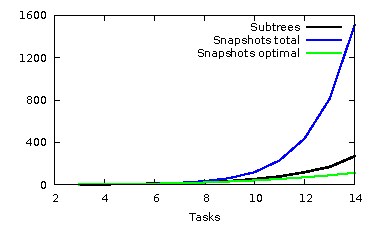
\includegraphics[scale=.8]{max.pdf}
      
      Maximum
    \end{column}
    \begin{column}{.5\textwidth}
      \centering
      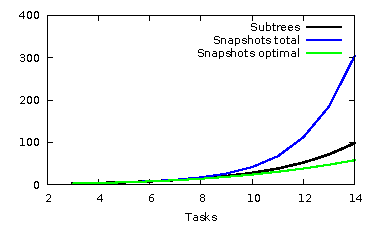
\includegraphics[scale=.8]{avg.pdf}
      
      Average
    \end{column}
  \end{columns}
\end{frame}

\begin{frame}
  \frametitle{Compressing the snapshot DAG}
  \begin{itemize}
  \item Optimal snapshot DAG allows (recursive) merging of some snapshots
  \item LEAF snapshot DAG prevents us from merging because the run times are not the same for some snapshots \todo{Verbessern!}
  \end{itemize}
\end{frame}

\subsection{Conjectures}

\begin{frame}
  \frametitle{Optimal strategies --- conjectures}
  \begin{itemize}
  \item \emph{In the beginning}, as many topmost task as possible shall be scheduled
    
    \note{Itermediate snapshots (in the optimal schedule) \emph{might} have fewer topmost task than possible scheduled}
  \item If the scheduler has a choice, it shall pick a topmost task, if available
  \item If only non-top tasks are scheduled, we can exchange any one with a topmost task and can obtain a better run time
  \end{itemize}
\end{frame}

\subsection{Particular classes of intrees}

\begin{frame}
  \frametitle{Degenerate intrees}
  \begin{itemize}
  \item On each level, at most one task has predecessors
  \item Uniquely determined by their profile
  \end{itemize}
  \begin{theorem}
    Degenerate intrees are optimally scheduled by HLF.
  \end{theorem}
  \begin{proof}
    \begin{itemize}
    \item Assert that for degenerate intree $I$, two tasks $z_1, z_2$ with $level(z_1) \geq level(z_2)$: 
      $T^*_{x,y,z_1}(I \cup \left\{ z_1 \right\}) \geq
      T^*_{x,y,z_2}(I \cup \left\{ z_2 \right\})$
    \item Induction over the number of tasks, comparing $T_{HLF}(I)$ to $T_{x',y',z'}(I)$
    \end{itemize}
  \end{proof}
\end{frame}

\begin{frame}
  \frametitle{Parallel chains}
  \begin{itemize}
  \item Each task, except the root, has at most one predecessor
  \item Parallel chains with up to 27 tasks are optimally scheduled by HLF
  \end{itemize}
\end{frame}

\begin{frame}
  \frametitle{Degenerate intrees and parallel chains --- outcome}
  \begin{itemize}
  \item HLF is deterministic for these classes \dots
  \item \dots and needs remarkably less snapshots than LEAF
  \item Example: Number of snapshots for degenerate binary trees
    \begin{center}
      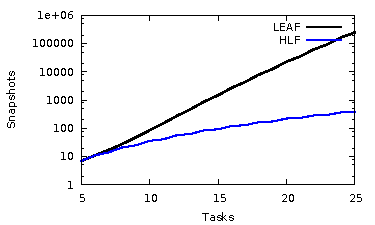
\includegraphics{deg_intrees.pdf}
    \end{center}
  \item Analogous results for parallel chains
  \end{itemize}
\end{frame}

\begin{frame}
  \frametitle{Improving LEAF with conjectures}
  \begin{block}{SCLEAF}
    \begin{itemize}
    \item Simple LEAF scheduler, but \dots
    \item \dots using HLF when encountering degenerate intrees or parallel chains \dots
    \item \dots restricts to snapshots where as many topmost task as possible are scheduled
    \end{itemize}
  \end{block}
  \begin{center}
    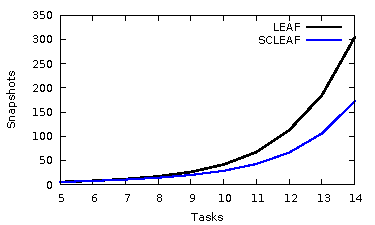
\includegraphics{scleaf.pdf}
  \end{center}
\end{frame}

\section{Program}

\begin{frame}
  \frametitle{Practical results}
  \begin{itemize}
  \item Excluding equivalent snapshots speeds up the program by at least factor 3 (for intrees with 11 or more tasks)
  \item Computing optimal schedules for all intrees with up to 15 tasks in 11 minutes and less than 2Gb of main memory
  \item More tasks require too much memory
  \item Computing optimal schedules for non-trivial intrees with 19 tasks takes one day
  \item Using Boost Rational to represent expectancies as fractions requires slightly more time and memory
  \item Using GMP to represent expectancies as fractions requires roughly doubles time and increases memory consumption by roughly 40\%
  \end{itemize}
\end{frame}

\end{document}

%%% Local Variables: 
%%% mode: latex
%%% TeX-master: t
%%% End: 
